\chapter{Results}
\label{chapter:results}
Two types of results are presented in this chapter: Screenshots showing different visual aspects of the system and benchmarks focusing on the achieved performance.

\section{Screenshots}
Screen shots from the implemented system are described and presented in each subsection below.

\begin{figure}[h]
  \centering
  \begin{subfigure}[bt]{0.9\textwidth}
    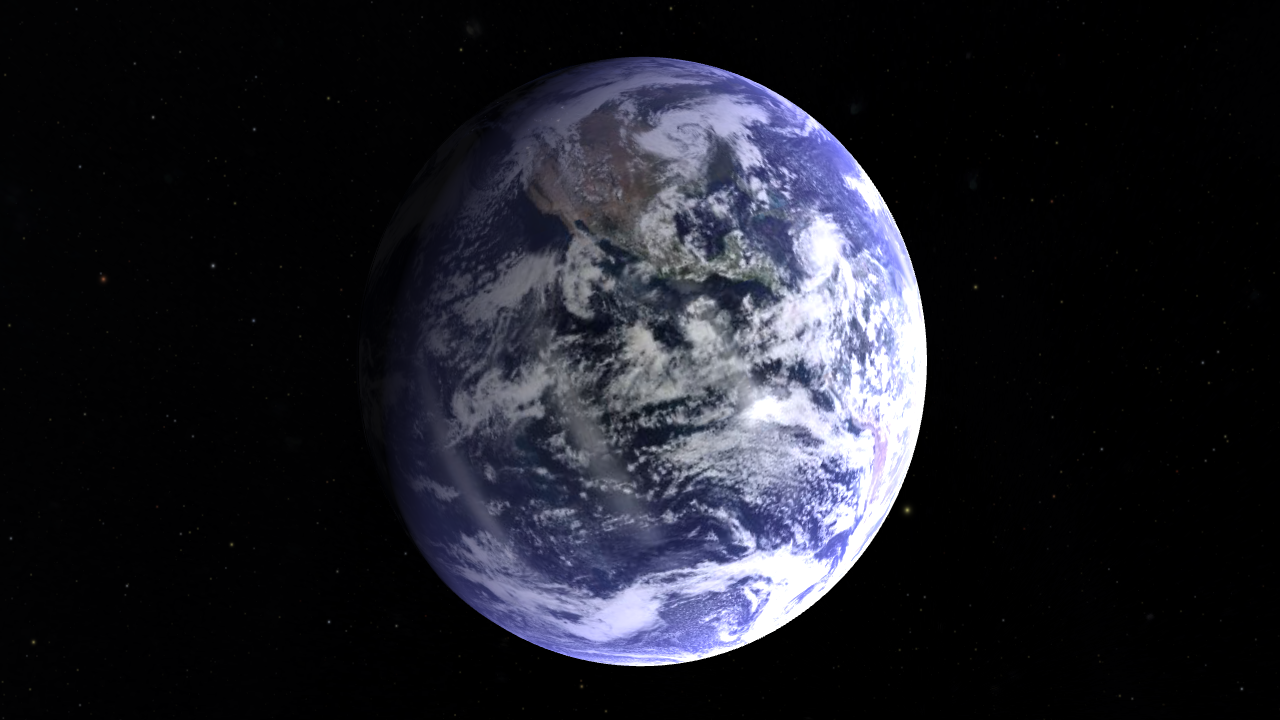
\includegraphics[width=\textwidth]{figures/appendices/screenshots/specular_earth.png}
    \caption{Shaded Earth rendered with Nasa Gibs VIIRS daily image.}
  \end{subfigure}
\end{figure}

\clearpage
\subsection{Water Masking}
\FloatBarrier
Earth rendered with a water mask layer enhancing specular contrasts between land and water.
\begin{figure}[h]
    \centering
    \begin{subfigure}[bt]{0.9\textwidth}
        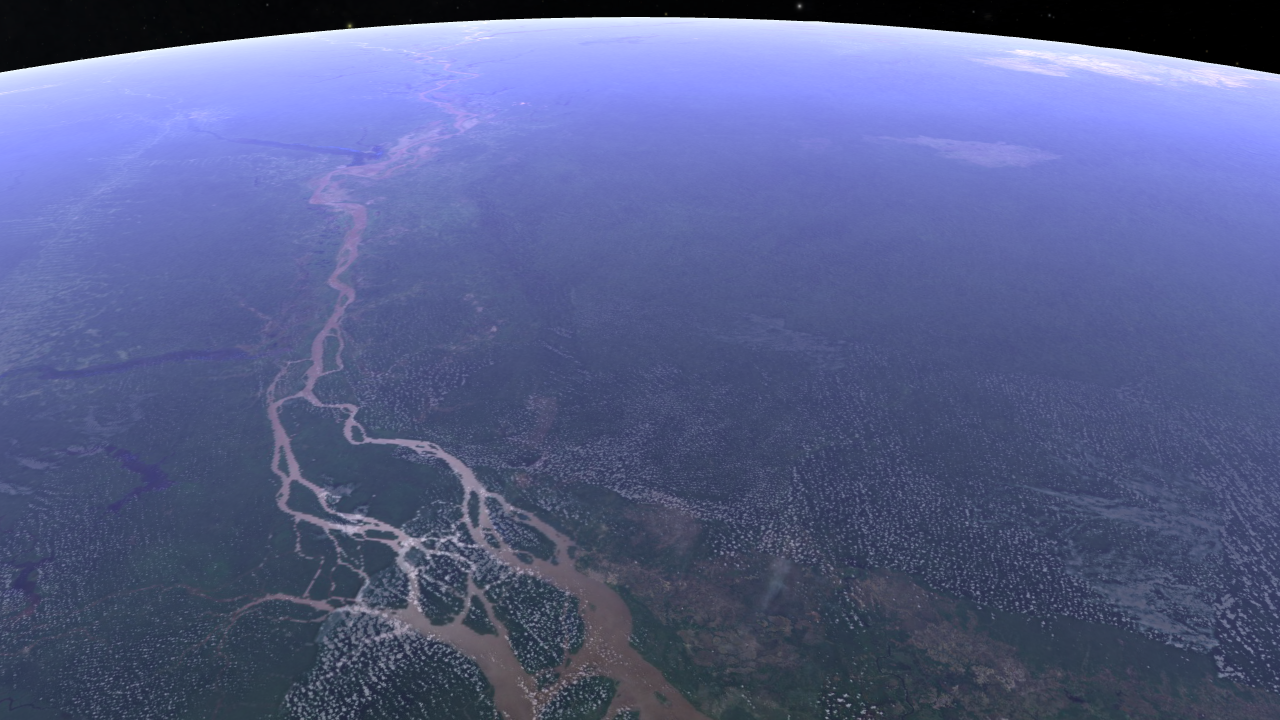
\includegraphics[width=\textwidth]{figures/appendices/screenshots/specular_brazil.png}
        \caption{Suns's specular reflection in Amazon River.}
    \end{subfigure}
    \begin{subfigure}[bt]{0.9\textwidth}
        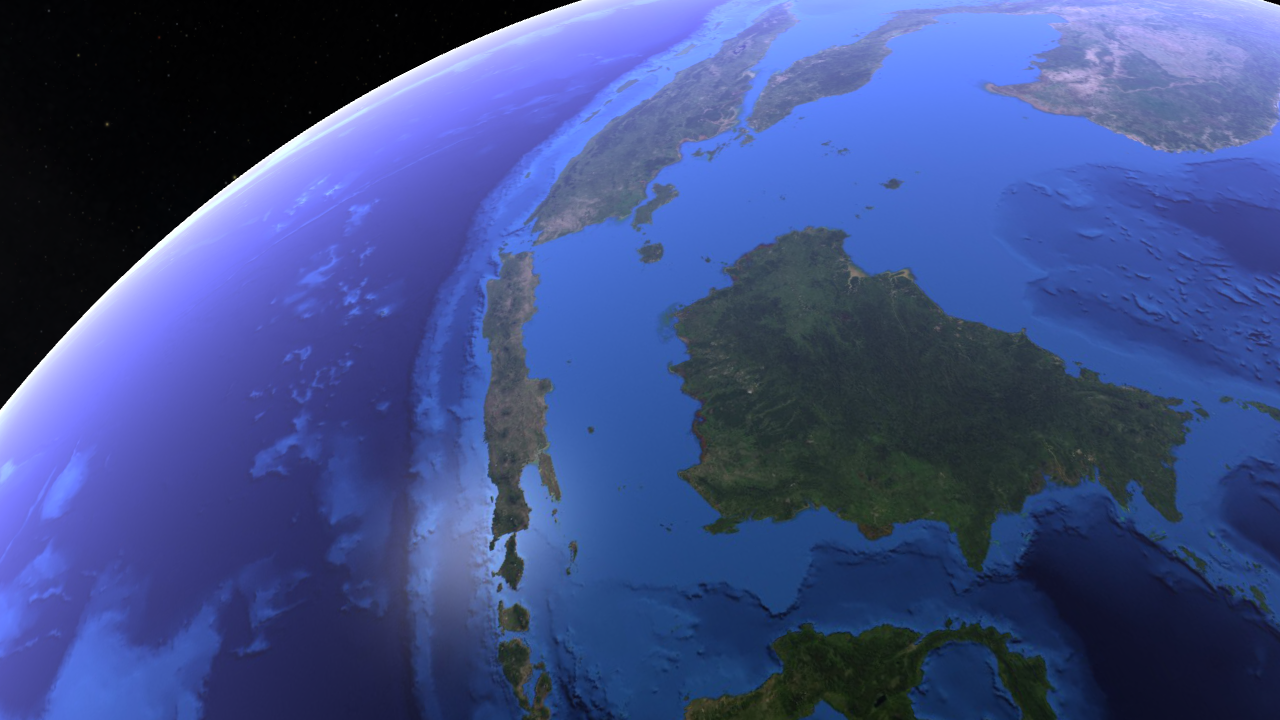
\includegraphics[width=\textwidth]{figures/appendices/screenshots/specular_indonesia.png}
        \caption{Sun's specular reflection around Bali, Indonesia.}
    \end{subfigure}
    \caption{Shaded globe using using water mask texture}
\end{figure}

\clearpage
\subsection{Chunk Bounding Volumes}
\FloatBarrier
Bounding polyhedra are calculated on the fly for each chunk, taking onto consideration any currently enabled height dataset. These bounding volumes are then used for by culling algorithms. Figure \ref{fig:boundingvolume} shows how smaller, more planar chunks can be encapsulated more tightly than large chunks by a polyhedron shape.
\begin{figure}[h]
    \centering
    \begin{subfigure}[bt]{0.45\textwidth}
        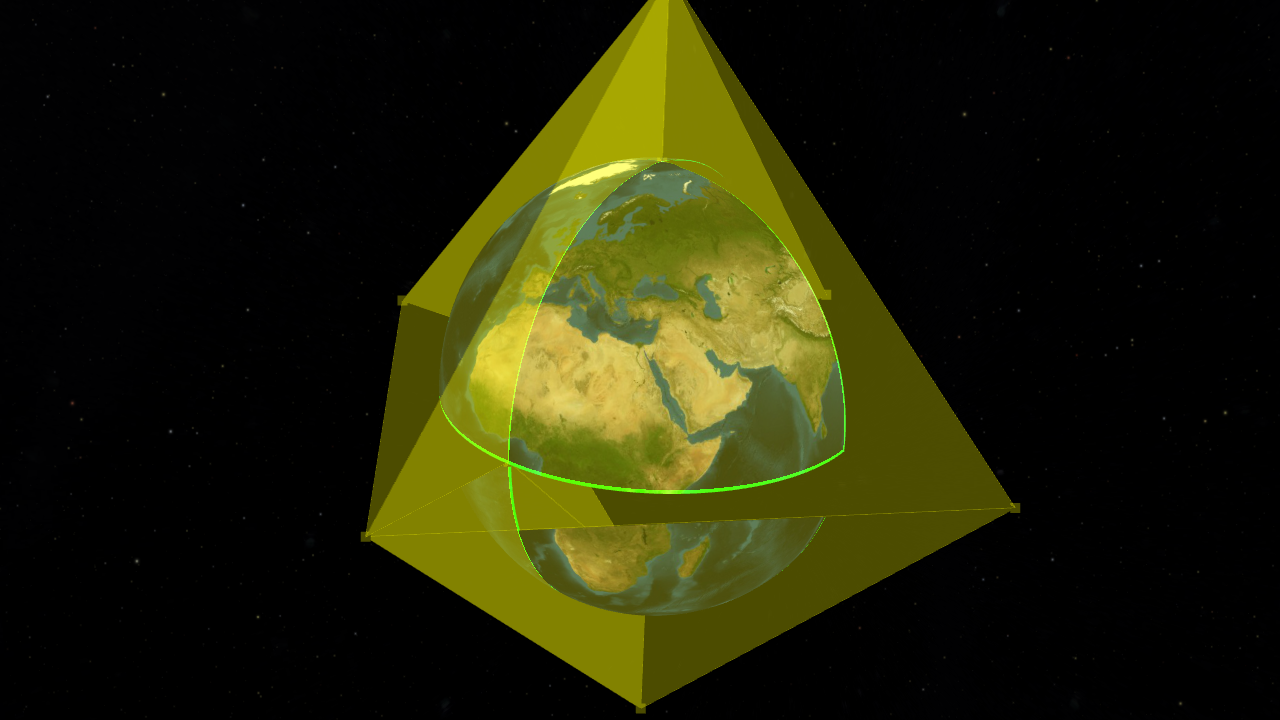
\includegraphics[width=\textwidth]{figures/results/culling/bbox_earth.png}
        \caption{Earth}
    \end{subfigure}
    \begin{subfigure}[bt]{0.45\textwidth}
        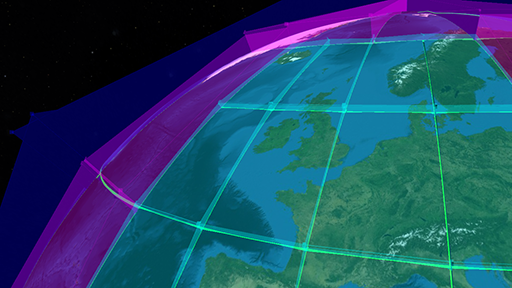
\includegraphics[width=\textwidth]{figures/results/culling/bbox_europe.png}
        \caption{Europe}
    \end{subfigure}
    \begin{subfigure}[bt]{0.45\textwidth}
        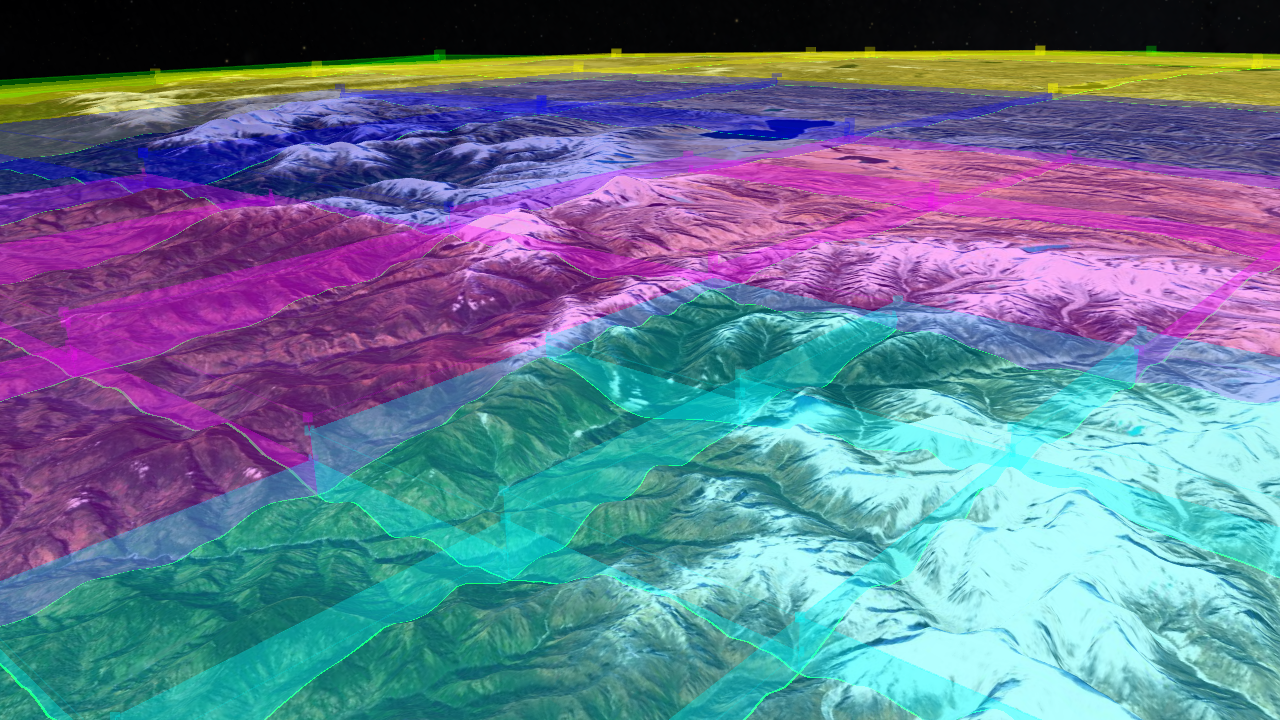
\includegraphics[width=\textwidth]{figures/results/culling/bbox_himalaya3.png}
        \caption{Himalaya mountain ridge}
    \end{subfigure}
    \begin{subfigure}[bt]{0.45\textwidth}
        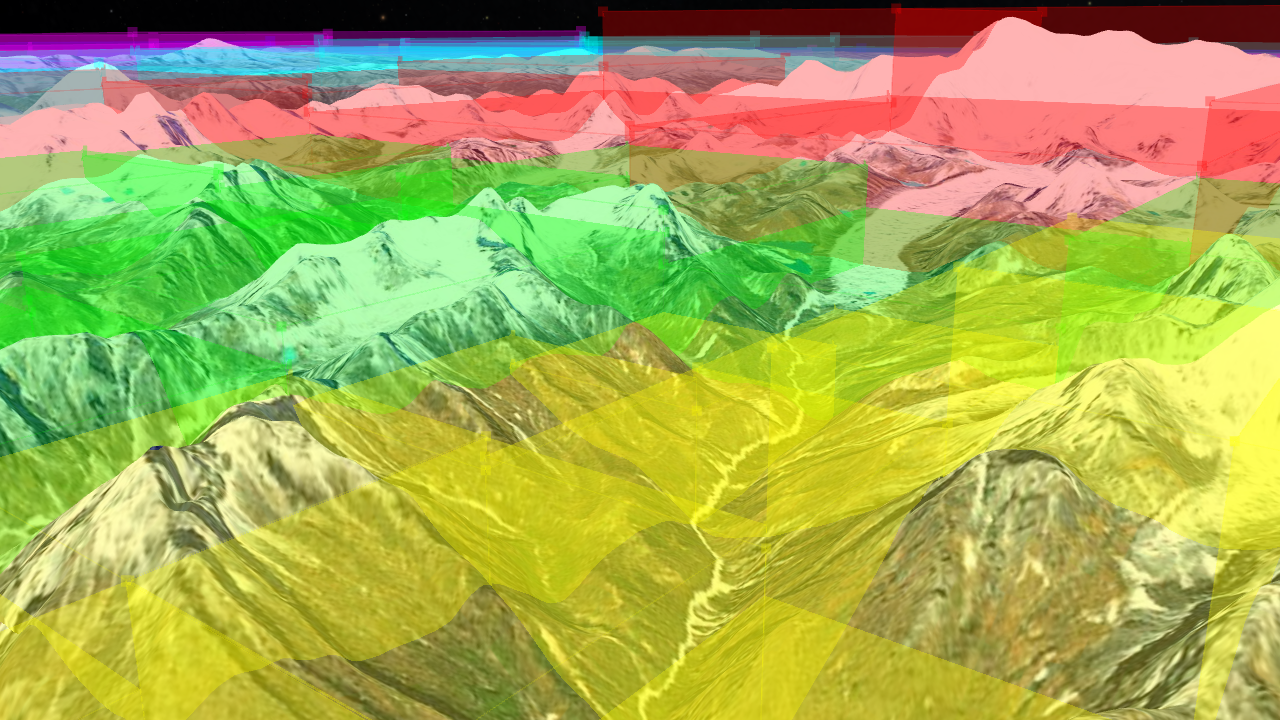
\includegraphics[width=\textwidth]{figures/results/culling/bbox_himalaya.png}
        \caption{Himalayan valley}
    \end{subfigure}
    \caption{Bounding volumes for each chunk are calculated for each chunk.}
    \label{fig:boundingvolume}
\end{figure}


\clearpage
\section{Benchmarking}
\FloatBarrier
This section goes through how the final implementation results in a software that solves the proposed objectives. Section (ref screenshots) \todo{ref} includes screenshots showing the globe browsing in use.

The benchmarks were done using the computer specified in table \ref{table:benchmark host}.

\begin{table}[h]
  \centering
  \caption[]{Computer used for Benchmarking}
    \label{table:benchmark host}
  \begin{tabular}{| r l |}
    \hline
      \textbf{Computer Model:}  & MacBook Pro (15'' early 2011) \\
      \textbf{Processor:}       & 2GHz Intel Core i7 \\
      \textbf{RAM:}             & 8 GB 1333MHz DDR3 RAM \\
      \textbf{Graphics:}        & AMD Radeon HD 6490M 256 MB \\
    \hline
  \end{tabular}
\end{table}



\clearpage
\subsection{Top Down Views}
\FloatBarrier
The chunk rendering algorithm was evaluated for a top down view at different distances to the ground. The settings for the evaluation are presented in Table \ref{table:settingstopdown}. The camera views for the evaluation points are shown in Figure \ref{fig:topdown} and the results are presented in Figure \ref{fig:topdowngraph1}.
\begin{table}[h]
  \centering
  \caption[]{Globe rendering settings for top down view benchmark}
    \label{table:settingstopdown}
  \begin{tabular}{| r l |}
    \hline
      \textbf{Globe:}             & Earth \\
      \textbf{Map datasets:}      & HeightLayers = [GCS\_Elevation \cite{worldelevation3d}] \\
                                  & ColorLayers = [ESRI Imagery World 2D \cite{imageryworld2d}] \\
      \textbf{LOD Scale factor:}  & 10.0 \\
      \textbf{Chunk Selction:}    & By distance \\
      \textbf{Culling:}           & Frustum culling, Horizon culling \\
      \textbf{Level blending:}    & Enabled \\
      \textbf{Camera View:}       & Facing down, varying altitudes\\
    \hline
  \end{tabular}
\end{table}

\begin{figure}[h]
    \centering
    \begin{subfigure}[bt]{0.31\textwidth}
        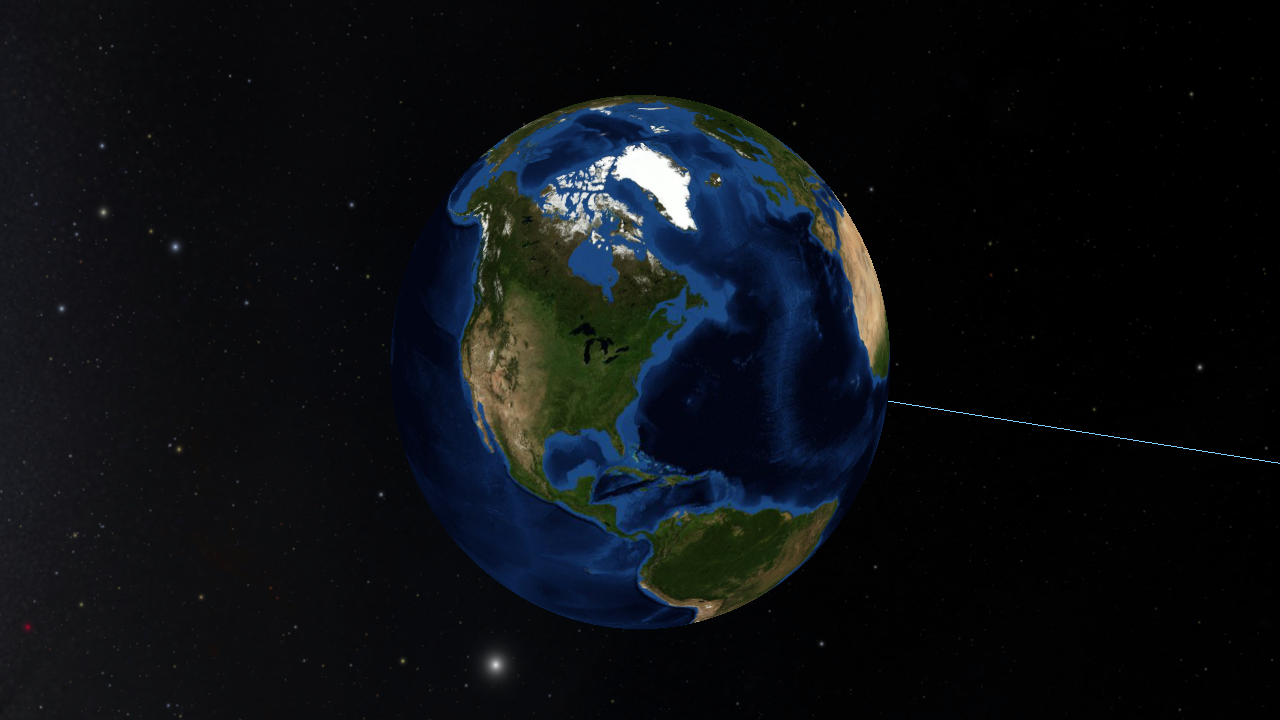
\includegraphics[width=\textwidth]{figures/results/topdown/topdown5.png}
        \caption{Earth}
    \end{subfigure}
    ~
    \begin{subfigure}[bt]{0.31\textwidth}
        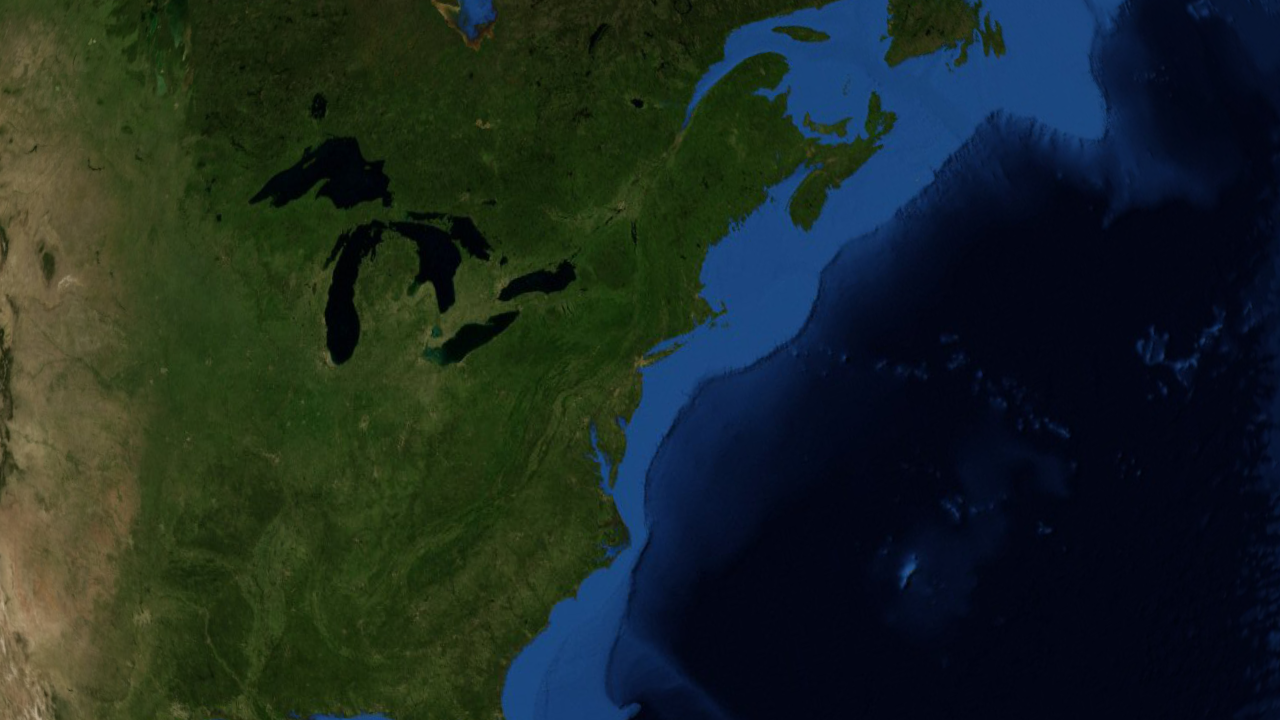
\includegraphics[width=\textwidth]{figures/results/topdown/topdown4.png}
        \caption{East America}
    \end{subfigure}
    ~
    \begin{subfigure}[bt]{0.31\textwidth}
        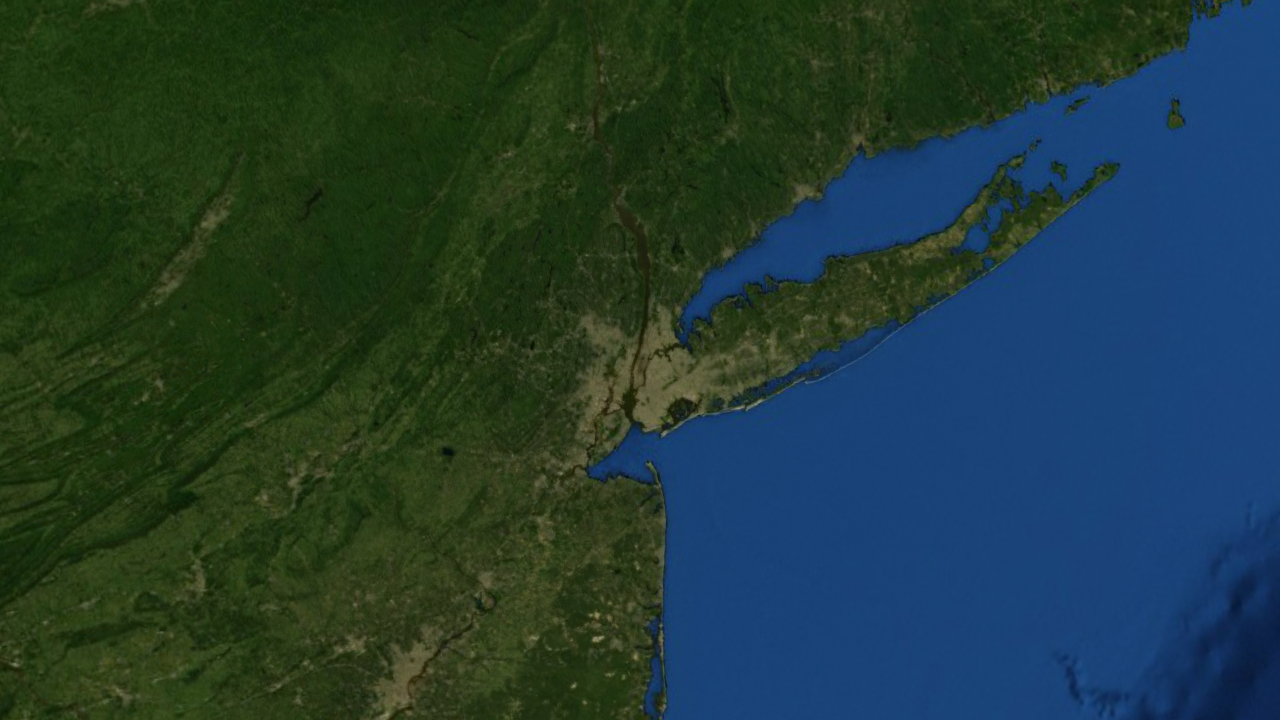
\includegraphics[width=\textwidth]{figures/results/topdown/topdown3.png}
        \caption{New York City}
    \end{subfigure}
    ~
    \begin{subfigure}[bt]{0.31\textwidth}
        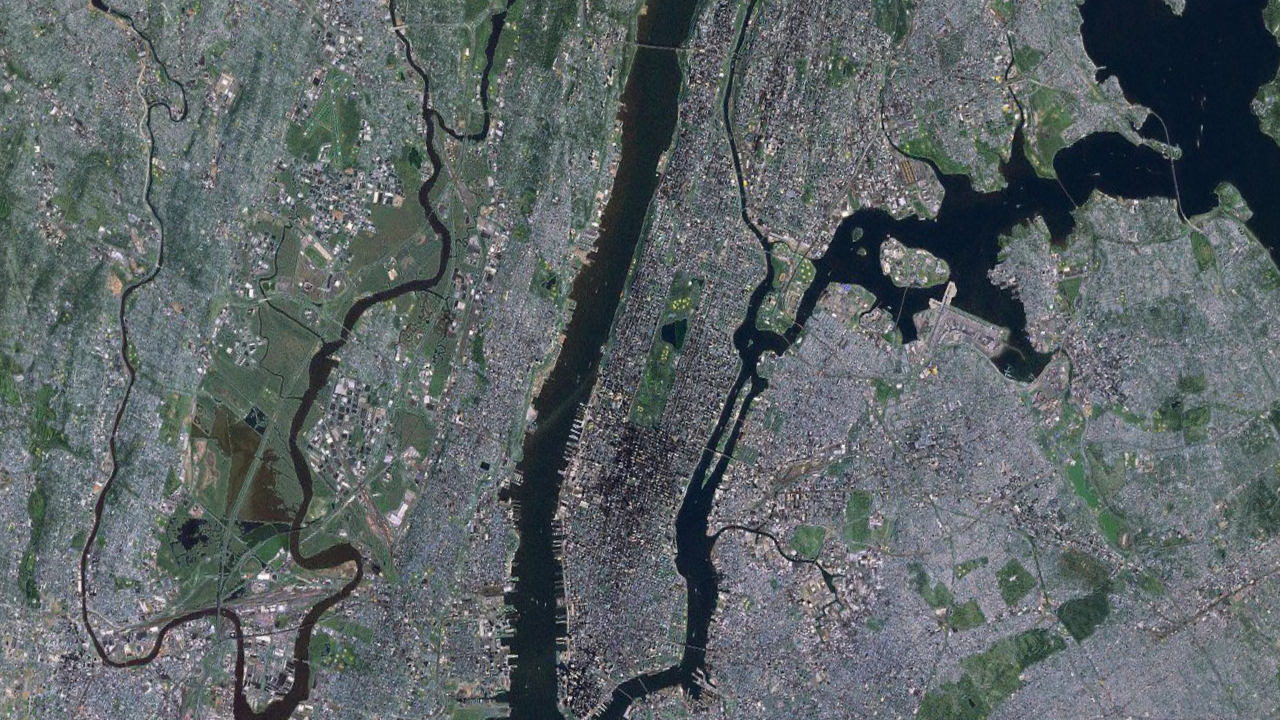
\includegraphics[width=\textwidth]{figures/results/topdown/topdown2.png}
        \caption{Manhattan}
    \end{subfigure}
    ~
    \begin{subfigure}[bt]{0.31\textwidth}
        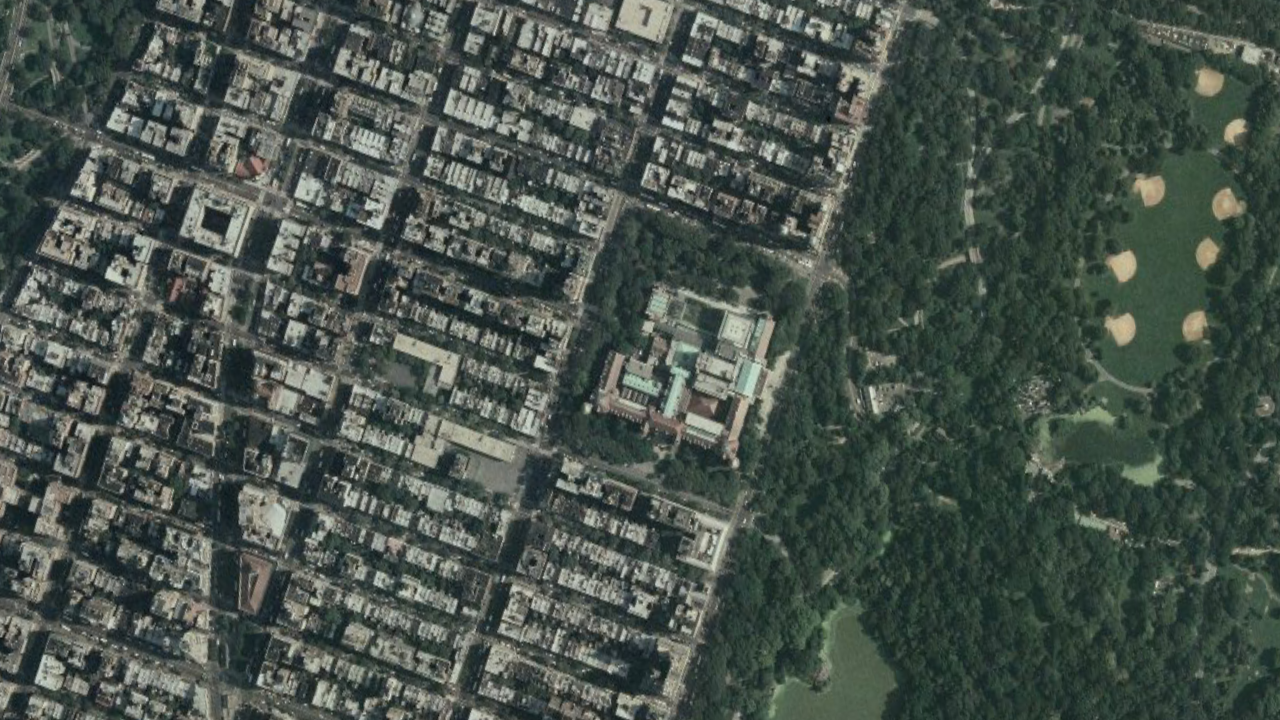
\includegraphics[width=\textwidth]{figures/results/topdown/topdown1.png}
        \caption{Central Park}
    \end{subfigure}
    \caption{Top down views of Earth at different altitudes}
    \label{fig:topdown}
\end{figure}

\begin{figure}[h]
\begin{tikzpicture}
    \begin{axis}[
        width  = 1.0*\textwidth,
        height = 12cm,
        major x tick style = transparent,
        ybar=2*\pgflinewidth,
        bar width=8pt,
        ymajorgrids = true,
        %ylabel = {Number of},
        symbolic x coords={Earth, East America, NYC, Manhattan, Central Park},
        xtick = data,
        scaled y ticks = false,
        enlarge x limits=0.25,
        ymin=0,
        legend cell align=left,
        legend style={
                at={(0.43, 0.66)},
                anchor=south east,
                column sep=1ex
        }
    ]

      \addplot[style={chunks_color,fill=chunks_color,mark=none}]
        coordinates { (Earth, 10) (East America, 70) (NYC, 70) (Manhattan, 110) (Central Park, 142) };

      \addplot[style={leafs_color,fill=leafs_color,mark=none}]
        coordinates { (Earth, 8) (East America, 53) (NYC, 53) (Manhattan, 83) (Central Park, 107) };
      
      \addplot[style={rendered_color,fill=rendered_color,mark=none}]
        coordinates { (Earth, 7) (East America, 14) (NYC, 13) (Manhattan, 17) (Central Park, 11) };

      \addplot[style={globe_render_time,fill=globe_render_time,mark=none}]
        coordinates { (Earth, 17) (East America, 20) (NYC, 20) (Manhattan, 21) (Central Park, 21) };

      \addplot[style={frame_render_time,fill=frame_render_time,mark=none}]
        coordinates { (Earth, 1.1) (East America, 3.4) (NYC, 3.5) (Manhattan, 5) (Central Park, 5.6) };

      \legend{Chunks, Leaf chunks, Rendered chunks, Frame time [ms], Globe render time [ms]}

    \end{axis}
\end{tikzpicture}
\caption{As the camera descends towards the ground looking straight down, the chunk tree grows but the number of rendered chunks remains relatively constant due to culling.}
\label{fig:topdowngraph1}
\end{figure}



\clearpage
\subsection{Culling For Distance Based Chunk Selection}
\label{ch:culld}
\FloatBarrier
The culling algorithms frustum culling and horizon culling were compared and evaluated.
The settings used are provided in table \ref{table:cullingdsettings}. Note that LOD evaluation is done by distance. Figure \ref{fig:cullingdcam} shows the camera view evaluated. Figure \ref{fig:cullingd} shows an overview of the rendered chunks with the results shown in figure \ref{fig:topdowngraphd}.


\begin{table}[h]
  \centering
  \caption[]{Globe rendering settings for evaluation of culling with distance based chunk selection}
  \label{table:cullingdsettings}
  \begin{tabular}{| r l |}
    \hline
      \textbf{Globe:}             & Earth \\
      \textbf{Map datasets:}      & HeightLayers = [GCS\_Elevation \cite{worldelevation3d}] \\
                                  & ColorLayers = [ESRI Imagery World 2D \cite{imageryworld2d}] \\
      \textbf{LOD Scale factor:}  & 7.8 \\
      \textbf{Chunk Selction:}    & By distance \\
      \textbf{Culling:}           & \textbf{Evaluated} \\
      \textbf{Level blending:}    & Enabled \\
      \textbf{Camera View:}       & Looking towards western horizon\\
      \textbf{Location:}          & New York, New Jersey\\
    \hline
  \end{tabular}
\end{table}

\begin{figure}[h]
    \centering
    \begin{subfigure}[bt]{1.0\textwidth}
        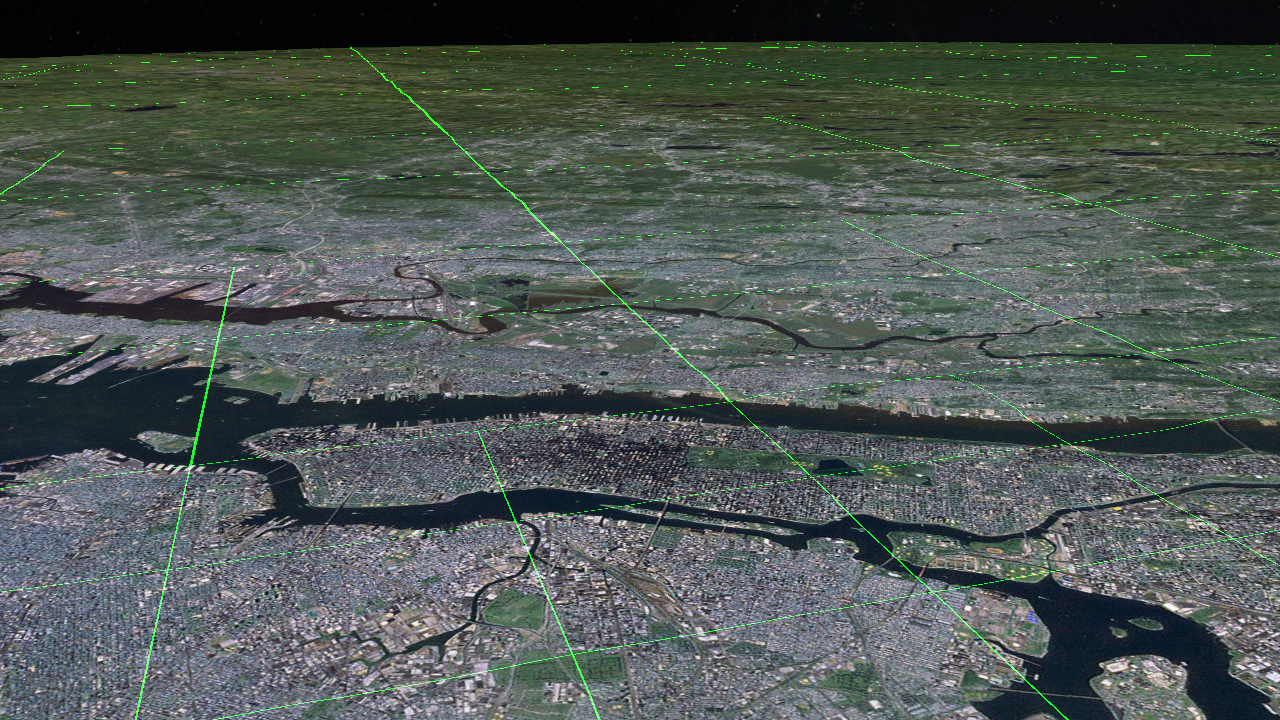
\includegraphics[width=\textwidth]{figures/results/culling/cam_d.png}
    \end{subfigure}
    \caption{Camera view looking over Brooklyn, Manhattan and New Jersey with distance based chunk selection. Chunk edges are shown to illustrate the difference in level of detail}
    \label{fig:cullingdcam}
\end{figure}

\clearpage
\begin{figure}[h]
    \centering
    \begin{subfigure}[t]{0.4\textwidth}
        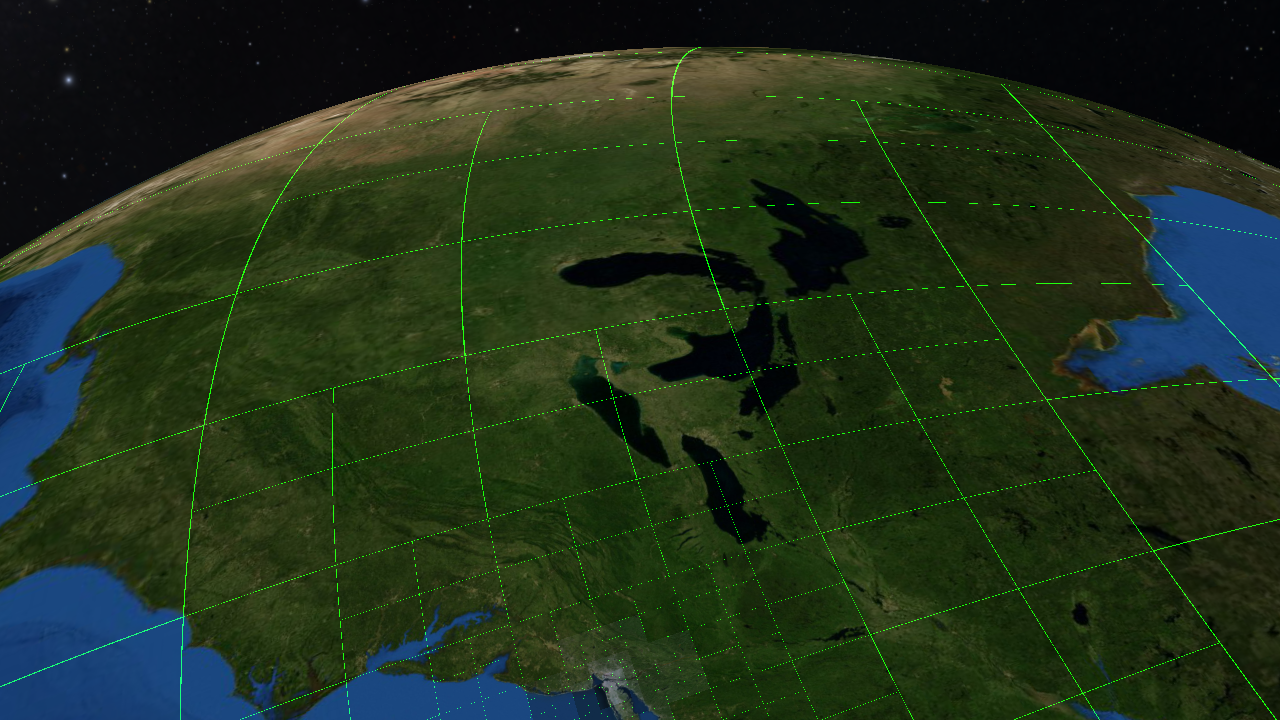
\includegraphics[width=\textwidth]{figures/results/culling/d.png}
        \caption{No culling}
    \end{subfigure}
    ~
    \begin{subfigure}[t]{0.4\textwidth}
        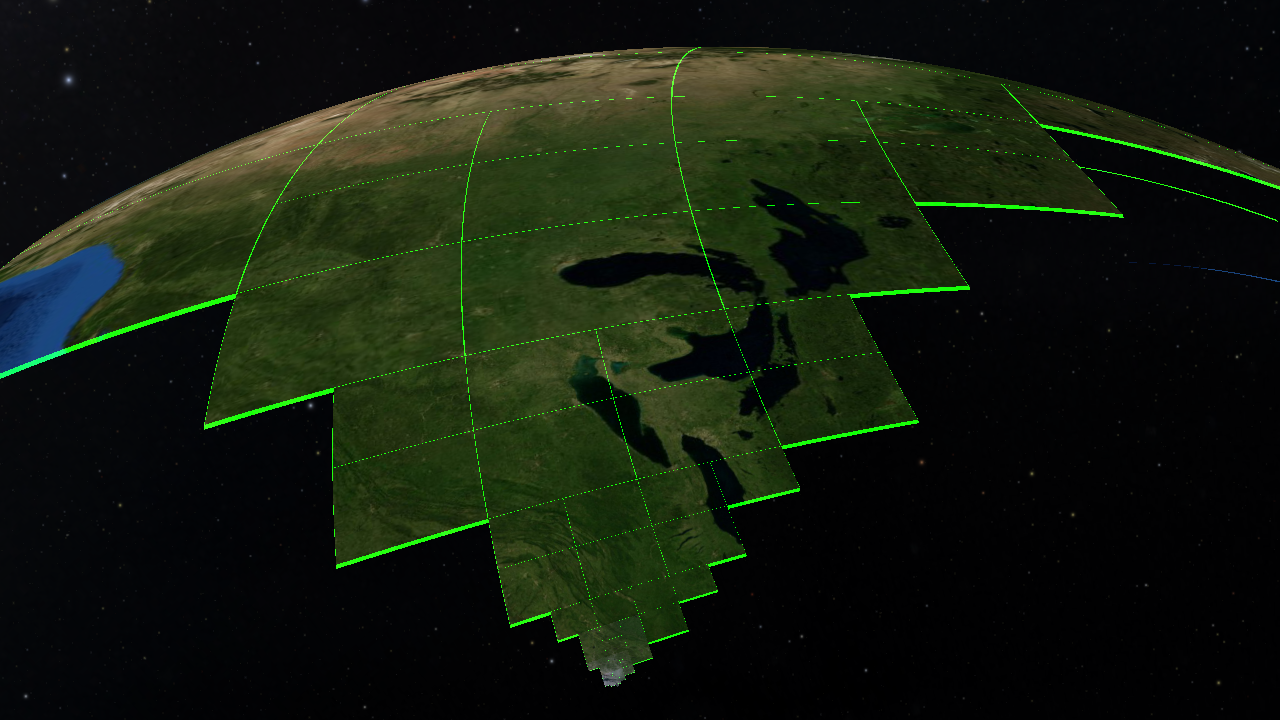
\includegraphics[width=\textwidth]{figures/results/culling/df.png}
        \caption{Frustum culling}
    \end{subfigure}
    ~
    \begin{subfigure}[t]{0.4\textwidth}
        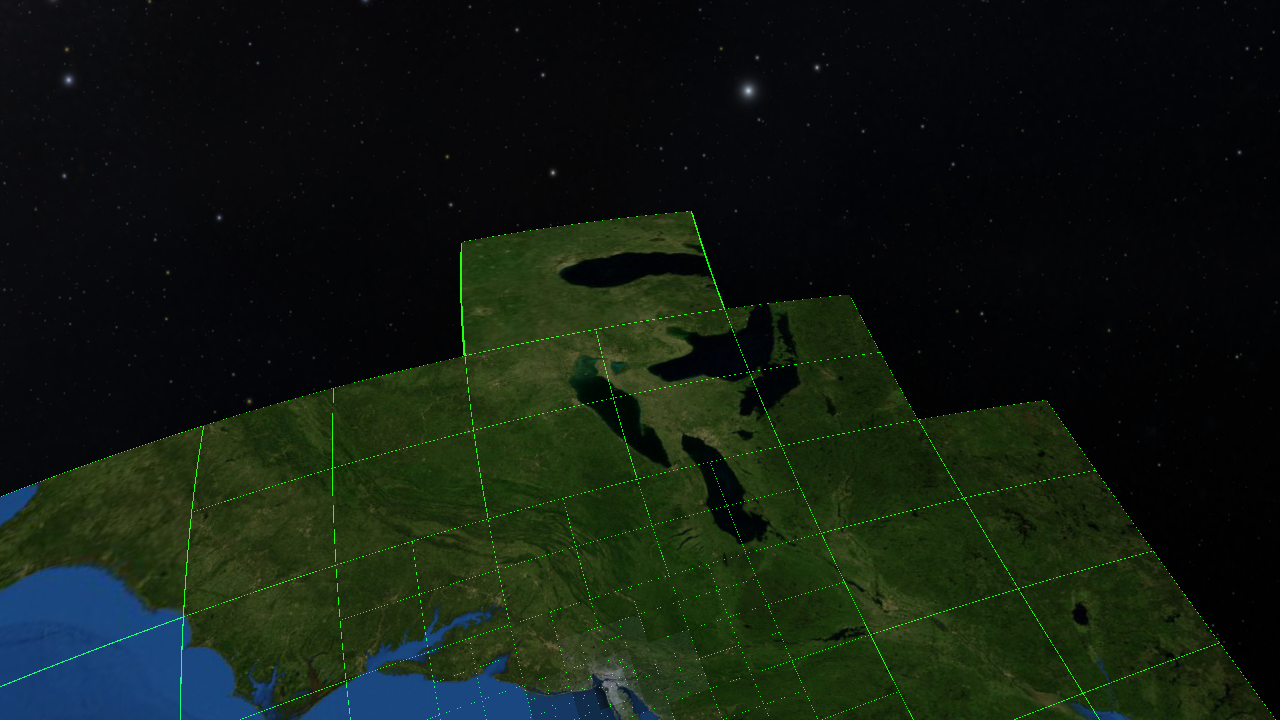
\includegraphics[width=\textwidth]{figures/results/culling/dh.png}
        \caption{Horizon culling}
    \end{subfigure}
    ~
    \begin{subfigure}[t]{0.4\textwidth}
        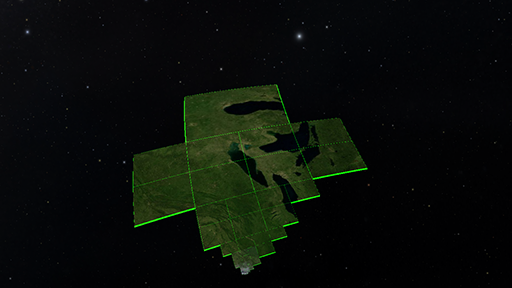
\includegraphics[width=\textwidth]{figures/results/culling/dhf.png}
        \caption{Frustum and horizon culling}
    \end{subfigure}
    \caption{Culling of chunks with distance based chunk selection}
    \label{fig:cullingd}
\end{figure}

\iffalse
\begin{table}[h]
\centering
\caption[]{Culling for projected area based chunk selection}
  \label{table:cullingd}
  \begin{tabular}{| r | c c c c |}
    \hline
      \textbf{Culling}            & \textbf{None}  & \textbf{Horizon} & \textbf{Frustum}  & \textbf{Both} \\ \hline
      \textbf{Chunk nodes}        & 514            & 390              & 214               & 154 \\ 
      \textbf{Leaf chunk nodes}   & 386            & 293              & 161               & 116 \\ 
      \textbf{Rendered chunks}    & 386            & 254              & 79                & 53 \\
      \textbf{Frame Time}         & 155 ms         & 53 ms            & 39 ms             & 28 ms \\
      \textbf{Globe render time}  & 119 ms         & 30 ms            & 14 ms             & 10 ms \\
    \hline
  \end{tabular}
\end{table}
\fi

\begin{figure}[h]
\begin{tikzpicture}
    \begin{axis}[
        width  = 1.0*\textwidth,
        height = 6.5cm,
        major x tick style = transparent,
        ybar=2*\pgflinewidth,
        bar width=8pt,
        ymajorgrids = true,
        %ylabel = {Number of},
        symbolic x coords={No Culling, Horizon Culling, Frustum Culling, Both},
        xtick = data,
        scaled y ticks = false,
        enlarge x limits=0.25,
        ymin=0,
        legend cell align=left,
        legend style={
                at={(0.99, 0.44)},
                anchor=south east,
                column sep=1ex
        }
    ]

      \addplot[style={chunks_color,fill=chunks_color,mark=none}]
        coordinates { (No Culling, 514) (Horizon Culling, 390) (Frustum Culling, 214) (Both, 154)};

      \addplot[style={leafs_color,fill=leafs_color,mark=none}]
        coordinates { (No Culling, 386) (Horizon Culling, 293) (Frustum Culling, 161) (Both, 116)};
      
      \addplot[style={rendered_color,fill=rendered_color,mark=none}]
        coordinates { (No Culling, 386) (Horizon Culling, 254) (Frustum Culling, 79) (Both, 53)};

      \addplot[style={frame_render_time,fill=globe_render_time,mark=none}]
        coordinates { (No Culling, 155) (Horizon Culling, 53) (Frustum Culling, 39) (Both, 28)};

      \addplot[style={globe_render_time,fill=frame_render_time,mark=none}]
        coordinates { (No Culling, 119) (Horizon Culling, 30) (Frustum Culling, 14) (Both, 10) };

      \legend{Chunks, Leaf chunks, Rendered chunks, Frame time [ms], Globe render time [ms]}

    \end{axis}
\end{tikzpicture}
\caption{The number of chunks effected by culling}
\label{fig:topdowngraphd}
\end{figure}

\clearpage
\subsection{Culling For Projected Area Based Chunk Selection}
\label{ch:culla}

\FloatBarrier

Another test was conducted to evaluate the culling algorithms. Instead of using chunk selection based on camera distance, the projected area evaluation was used. The settings used are provided in table \ref{table:cullingasettings}. Figure \ref{fig:cullingacam} shows the camera view evaluated. Figure \ref{fig:cullinga} shows an overview of the rendered chunks with the results shown in figure \ref{fig:topdowngrapha}.

\begin{table}[h]
  \centering
  \caption[]{Globe rendering Settings for evaluation of culling with area based chunk selection}
  \label{table:cullingasettings}
  \begin{tabular}{| r l |}
    \hline
      \textbf{Globe:}             & Earth \\
      \textbf{Map datasets:}      & HeightLayers = [GCS\_Elevation \cite{worldelevation3d}] \\
                                  & ColorLayers = [ESRI Imagery World 2D \cite{imageryworld2d}] \\
      \textbf{LOD Scale factor:}  & 7.8 \\
      \textbf{Chunk Selction:}    & By projected area \\
      \textbf{Culling:}           & \textbf{Evaluated} \\
      \textbf{Level blending:}    & Enabled \\
      \textbf{Camera View:}       & Looking towards western horizon\\
      \textbf{Location:}          & New York, New Jersey\\
    \hline
  \end{tabular}
\end{table}

\begin{figure}[h]
    \centering
    \begin{subfigure}[bt]{1.0\textwidth}
        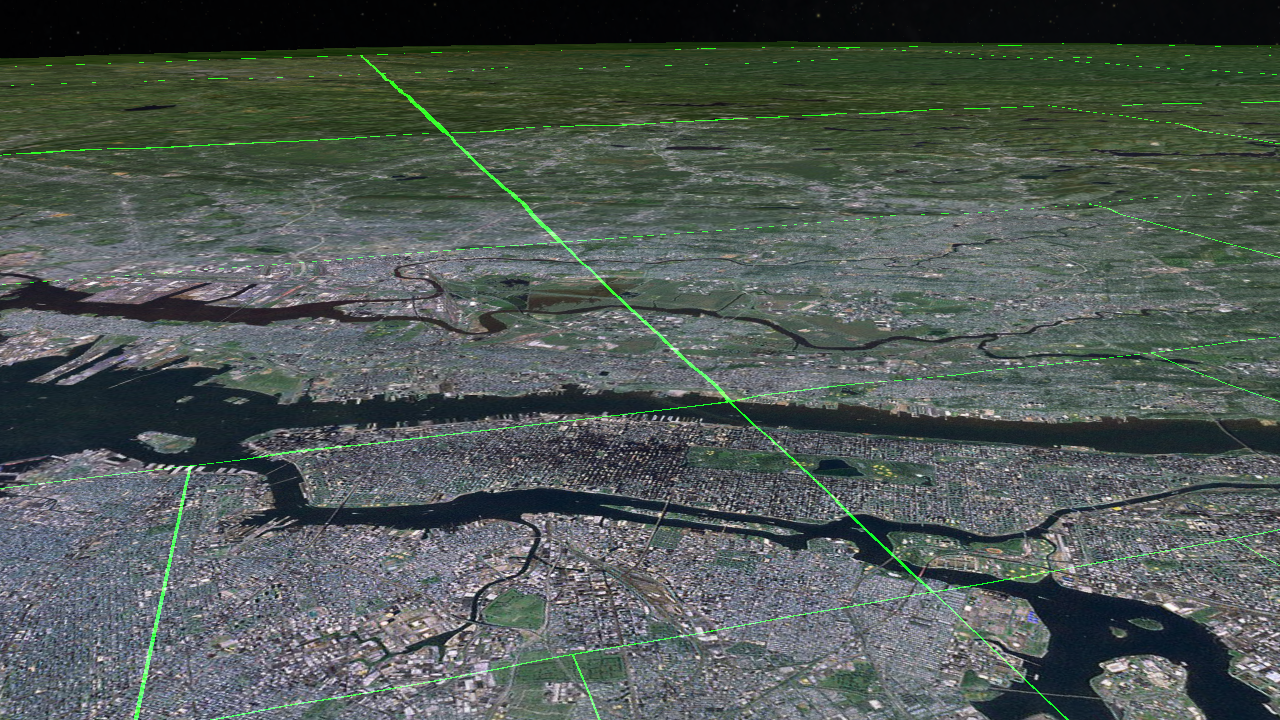
\includegraphics[width=\textwidth]{figures/results/culling/cam_a.png}
    \end{subfigure}
    \caption{Camera view looking over Brooklyn, Manhattan and New Jersey with projected area based chunk selection}
    \label{fig:cullingacam}
\end{figure}

\clearpage
\begin{figure}[h]
    \centering
    \begin{subfigure}[bt]{0.4\textwidth}
        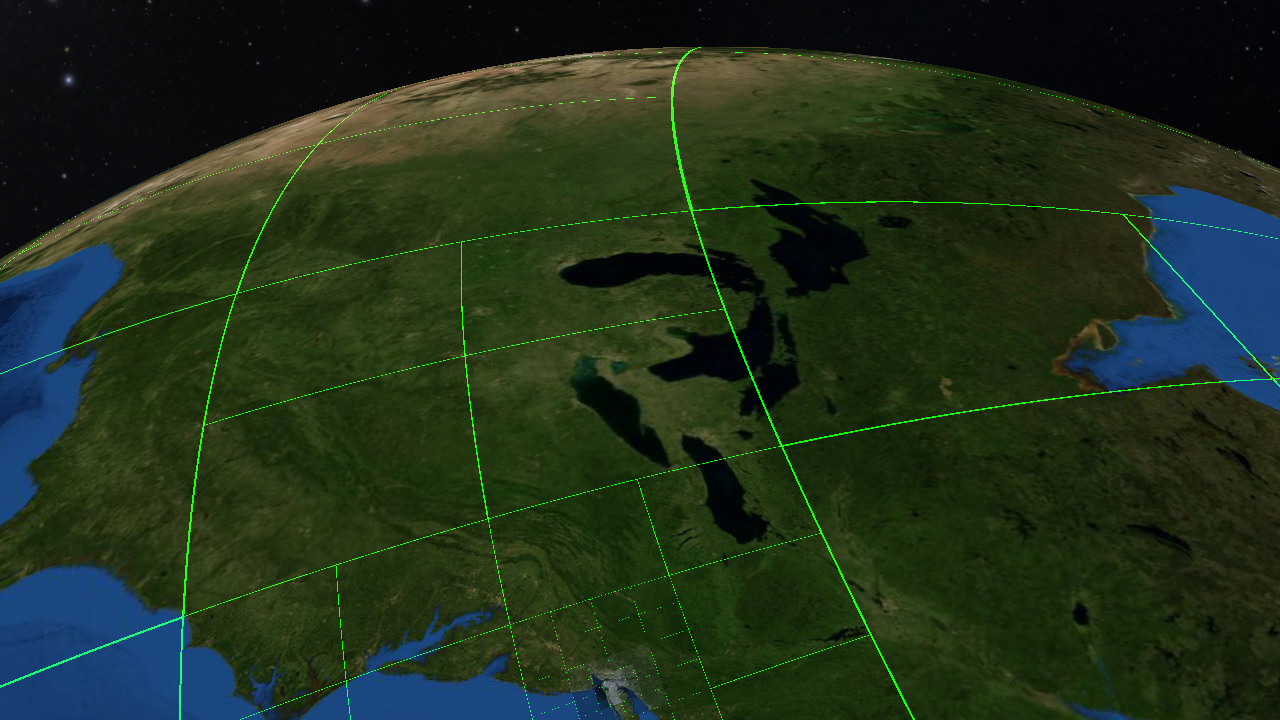
\includegraphics[width=\textwidth]{figures/results/culling/a.png}
        \caption{No culling}
    \end{subfigure}
    ~
    \begin{subfigure}[bt]{0.4\textwidth}
        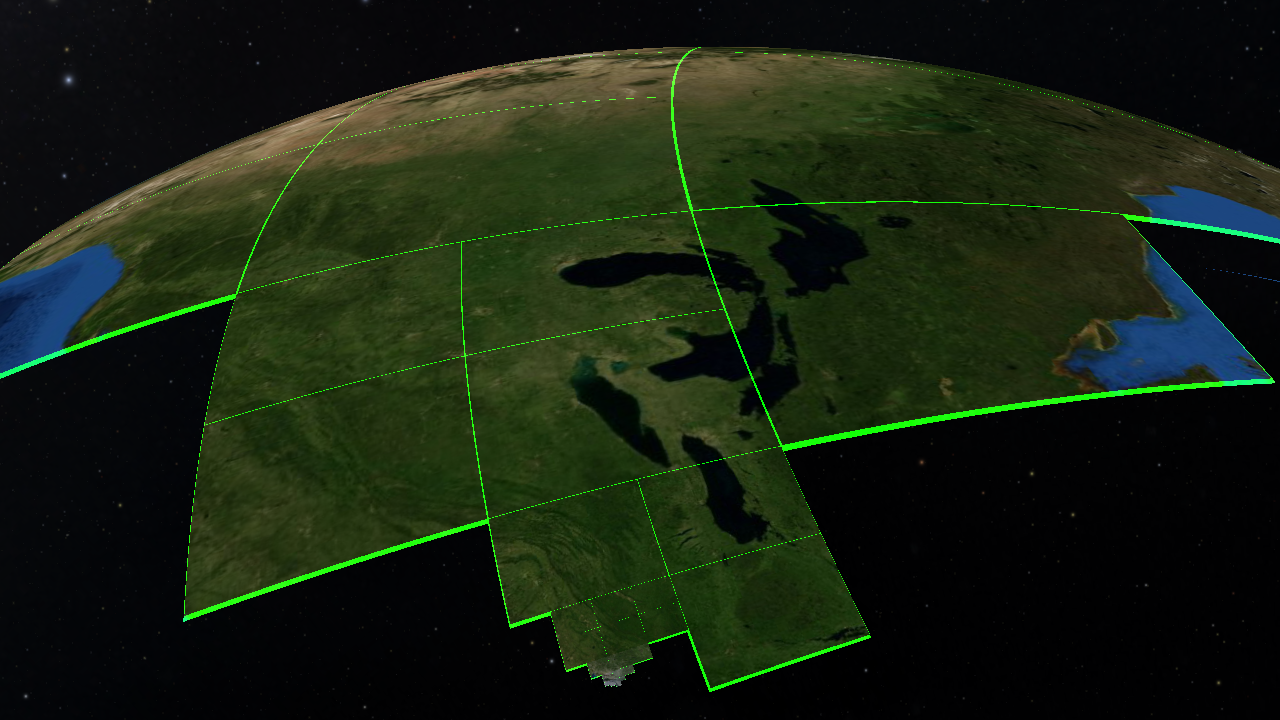
\includegraphics[width=\textwidth]{figures/results/culling/af.png}
        \caption{Frustum culling}
    \end{subfigure}
    ~
    \begin{subfigure}[bt]{0.4\textwidth}
        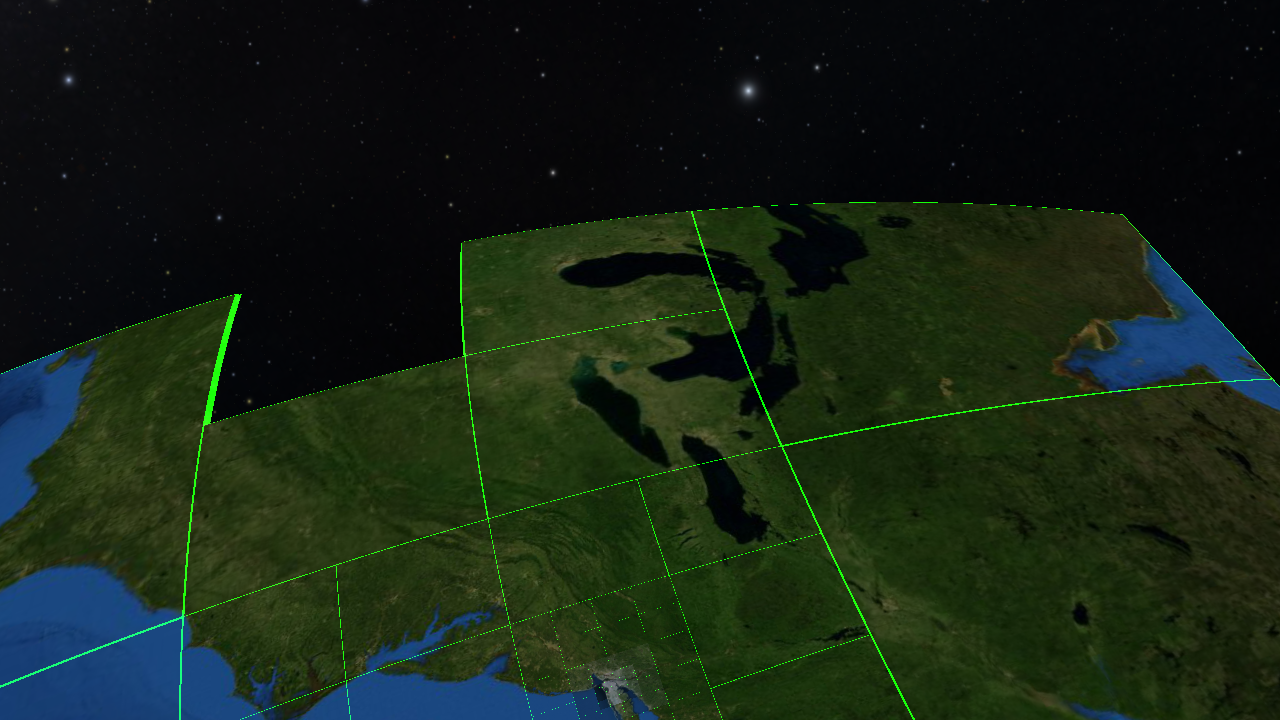
\includegraphics[width=\textwidth]{figures/results/culling/ah.png}
        \caption{Horizon culling}
    \end{subfigure}
    ~
    \begin{subfigure}[bt]{0.4\textwidth}
        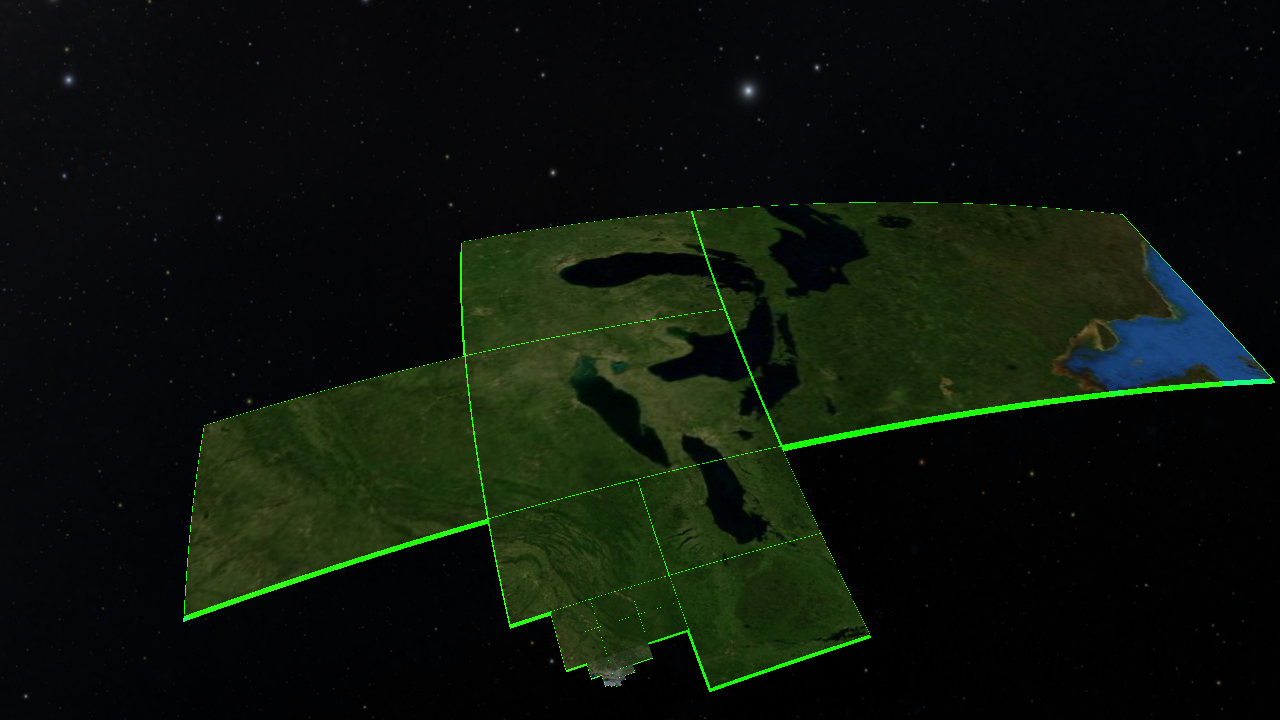
\includegraphics[width=\textwidth]{figures/results/culling/afh.png}
        \caption{Frustum and Horizon culling}
    \end{subfigure}
    \caption{Culling of chunks with area based chunk selection}
    \label{fig:cullinga}
\end{figure}

\iffalse
\begin{table}[h]
\centering
\caption[]{Projcted area based}
  \label{table:cullinga}
  \begin{tabular}{| r | c c c c |}
    \hline
      \textbf{Culling}            & \textbf{None} & \textbf{Horizon}  & \textbf{Frustum}  & \textbf{Both} \\ \hline
      \textbf{Chunk nodes}        & 270           & 202               & 134               & 94 \\ 
      \textbf{Leaf chunk nodes}   & 203           & 152               & 101               & 71 \\ 
      \textbf{Rendered chunks}    & 203           & 133               & 43                & 26 \\
      \textbf{Frame Time}         & 123 ms        & 41 ms             & 30 ms             & 23 ms \\
      \textbf{Globe render time}  & 62 ms         & 16 ms             & 7.9 ms            & 5.6 ms \\
    \hline
  \end{tabular}
\end{table}
\fi



\begin{figure}[h]
\begin{tikzpicture}
    \begin{axis}[
        width  = 1.0*\textwidth,
        height = 6.5cm,
        major x tick style = transparent,
        ybar=2*\pgflinewidth,
        bar width=8pt,
        ymajorgrids = true,
        %ylabel = {Number of},
        symbolic x coords={No Culling, Horizon Culling, Frustum Culling, Both},
        xtick = data,
        scaled y ticks = false,
        enlarge x limits=0.25,
        ymin=0,
        legend cell align=left,
        legend style={
                at={(0.995, 0.44)},
                anchor=south east,
                column sep=1ex
        }
    ]

      \addplot[style={chunks_color,fill=chunks_color,mark=none}]
        coordinates { (No Culling, 270) (Horizon Culling, 202) (Frustum Culling, 134) (Both, 94)};

      \addplot[style={leafs_color,fill=leafs_color,mark=none}]
        coordinates { (No Culling, 203) (Horizon Culling, 152) (Frustum Culling, 101) (Both, 71)};

      \addplot[style={rendered_color,fill=rendered_color,mark=none}]
        coordinates { (No Culling, 203) (Horizon Culling, 133) (Frustum Culling, 43) (Both, 26)};

      \addplot[style={frame_render_time,fill=globe_render_time,mark=none}]
        coordinates { (No Culling, 123) (Horizon Culling, 41) (Frustum Culling, 30) (Both, 23)};

      \addplot[style={globe_render_time,fill=frame_render_time,mark=none}]
        coordinates { (No Culling, 62) (Horizon Culling, 16) (Frustum Culling, 7.9) (Both, 5.6) };

      \legend{Chunks, Leaf chunks, Rendered chunks, Frame time [ms], Globe render time [ms]}

    \end{axis}
\end{tikzpicture}
\caption{The number of chunks effected by culling}
\label{fig:topdowngrapha}
\end{figure}

\clearpage
\subsection{LOD: Distance Based vs. Area Based}
\FloatBarrier

The benchmark results in section \ref{ch:culld} and \ref{ch:culla} were compared and evaluated in relation to each other. In figure \ref{fig:lodcomp} the two approaches are compared where both frustum culling and horizon culling were enabled.

\begin{figure}[h]
\begin{tikzpicture}
    \begin{axis}[
        width  = 0.9*\textwidth,
        height = 15cm,
        major x tick style = transparent,
        ybar=2*\pgflinewidth,
        bar width=15pt,
        ymajorgrids = true,
        ylabel = {},
        symbolic x coords={Distance based chunk selection, Area based chunk selection},
        xtick = data,
        scaled y ticks = false,
        enlarge x limits=0.55,
        ymin=0,
        legend cell align=left,
        legend style={
                at={(0.995, 0.74)},
                anchor=south east,
                column sep=1ex
        }
    ] 

      \addplot[style={chunks_color,fill=chunks_color,mark=none}]
        coordinates { (Distance based chunk selection, 154) (Area based chunk selection, 94) };

      \addplot[style={leafs_color,fill=leafs_color,mark=none}]
        coordinates { (Distance based chunk selection, 116) (Area based chunk selection, 71) };

      \addplot[style={rendered_color,fill=rendered_color,mark=none}]
        coordinates { (Distance based chunk selection, 53) (Area based chunk selection, 26) };

      \addplot[style={frame_render_time,fill=frame_render_time,mark=none}]
        coordinates { (Distance based chunk selection, 28) (Area based chunk selection, 23) };

      \addplot[style={globe_render_time,fill=globe_render_time,mark=none}]
        coordinates { (Distance based chunk selection, 10) (Area based chunk selection, 5.6) };

      \legend{Chunks, Leaf chunks, Rendered chunks, Frame time [ms], Globe render time [ms]}

    \end{axis}
\end{tikzpicture}
\caption{Comparison of Distance based - and Area based chunk selection}
\label{fig:lodcomp}
\end{figure}

\clearpage
\subsection{Switching Using Level Blending}
\label{section:res_switching}
\FloatBarrier
The visual result of using the distance based level blending is shown in Figure \ref{fig:blending2}.
\begin{figure}[h]
    \centering
    \begin{subfigure}[bt]{0.48\textwidth}
        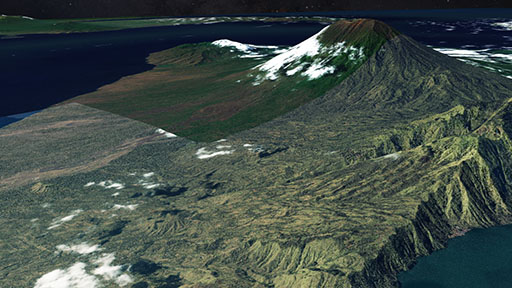
\includegraphics[width=\textwidth]{figures/results/blending/blending_bali2_disabled.jpg}
        \caption{Blending disabled}
    \end{subfigure}
    \begin{subfigure}[bt]{0.48\textwidth}
        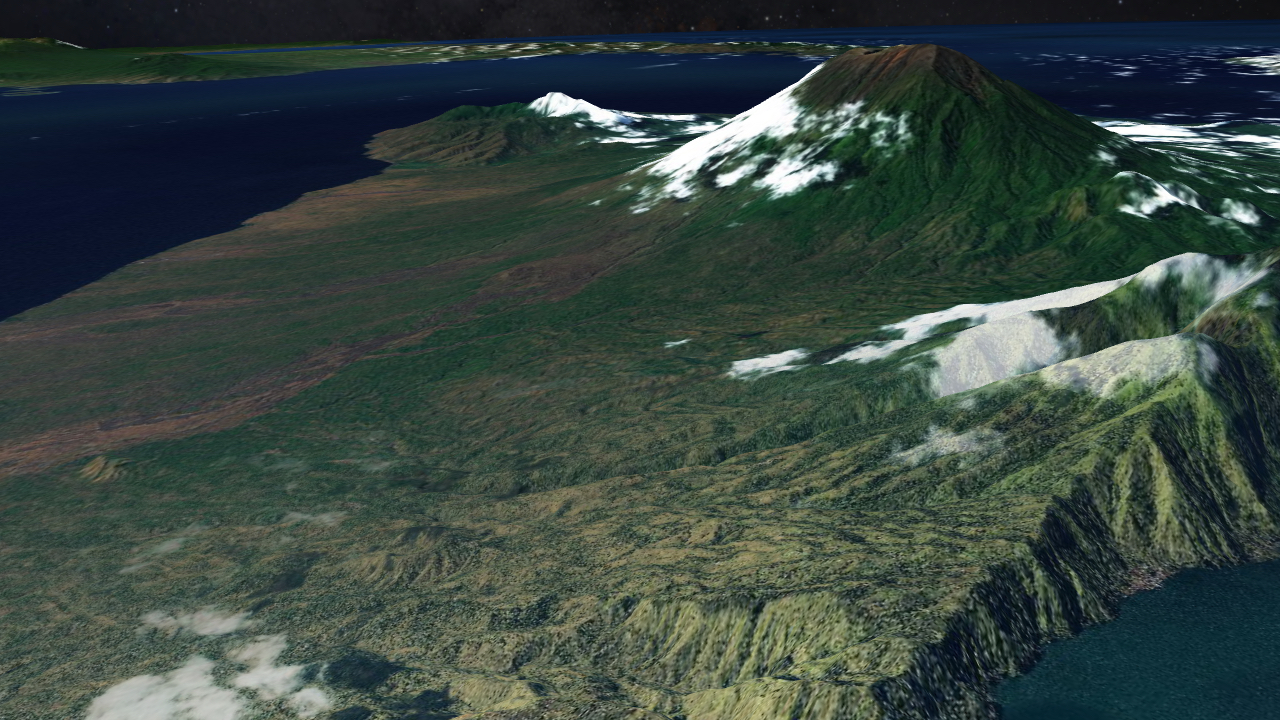
\includegraphics[width=\textwidth]{figures/results/blending/blending_bali2_enabled.jpg}
        \caption{Blending enabled}
    \end{subfigure}
    \caption{Comparison of using level blending and no blending. Notice level blending hides edges the underlying chunks}
    \label{fig:blending2}
\end{figure}

Table \ref{table:levelblending} shows the settings used to compare having level blending enabled and disabled. To show the penalty in texture detail that is payed for using level blending, the LOD scale factor was set low. Figure \ref{fig:blending} shows that the texture resolution becomes low enough to see the individual pixels when having a low LOD. The results in table \ref{table:resultblending} also show that figure \ref{fig:blendingdisabled} contains more visual information than \ref{fig:blendingenabled}. 

\begin{table}
  \centering
  \caption[]{Globe rendering settings used in benchmark}
    \label{table:levelblending}
  \begin{tabular}{| r l |}
    \hline
      \textbf{Globe:}             & Earth \\
      \textbf{Map datasets:}      & HeightLayers = [GCS\_Elevation \cite{worldelevation3d}] \\
                                  & ColorLayers = [ESRI Imagery World 2D \cite{imageryworld2d}] \\
      \textbf{LOD Scale factor:}  & 4.65 \\
      \textbf{Chunk Selction:}    & By distance \\
      \textbf{Culling:}           & Frustum culling, Horizon culling \\
      \textbf{Camera View:}       & Horizon \\
    \hline
  \end{tabular}
\end{table}

\begin{figure}[h]
    \centering
    \begin{subfigure}[bt]{0.48\textwidth}
        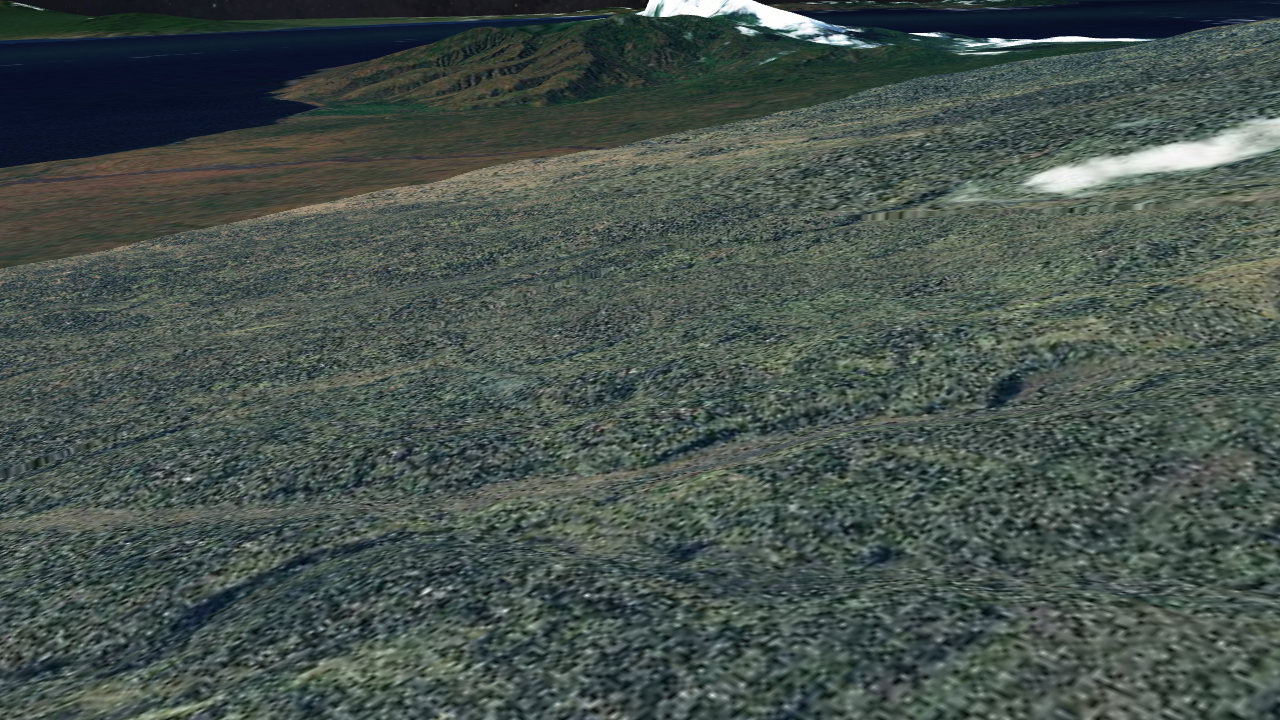
\includegraphics[width=\textwidth]{figures/results/blending/blending_bali_disabled.jpg}
        \caption{Blending disabled}
        \label{fig:blendingdisabled}
    \end{subfigure}
    \begin{subfigure}[bt]{0.48\textwidth}
        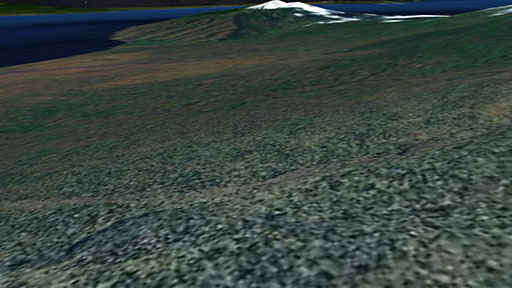
\includegraphics[width=\textwidth]{figures/results/blending/blending_bali_enabled.jpg}
        \caption{Blending enabled}
        \label{fig:blendingenabled}
    \end{subfigure}
    \caption{Comparison of level blending and no blending. The LOD scale factor is set low to show the resolution penalty of using blending}
    \label{fig:blending}
\end{figure}

\begin{table}
\centering
\caption[]{Level blending benchmarks. Comparing the disk space of a compressed JPEG image of both cases works as a heuristic to the information contained in each image}
  \label{table:resultblending}
  \begin{tabular}{| r | c c |}
    \hline
      \textbf{Figure \ref{fig:blending}}  & \textbf{No blending} & \textbf{Level blending} \\ \hline
      \textbf{Samples per fragment} & 1 & 3 \\ 
      \textbf{Avg. globe render time}  & 10.3 ms & 10.1 ms \\ 
      \textbf{Avg. frame time}  & 40 ms &  49 ms \\ 
      \textbf{Screenshot jpg size} & 1,1 MB & 0,7 MB \\
    \hline
  \end{tabular}
\end{table}

\clearpage
\subsection{Polar Pinching}
\label{section:res_polarpinching}
\FloatBarrier
The impact of polar pinching on the chunk tree was evaluated using both distance based chunk selection and area based chunk selection. The results are presented in figure \ref{fig:pincheval}.

\begin{table}[h]
  \centering
  \caption[]{Globe rendering settings for evaluation of polar pinching}
  \label{table:pinchingstart}
  \begin{tabular}{| r l |}
    \hline
      \textbf{Globe:}             & Earth \\
      \textbf{Map datasets:}      & HeightLayers = [GCS\_Elevation\cite{worldelevation3d}] \\
                                  & ColorLayers = [ESRI Imagery World 2D \cite{imageryworld2d}] \\
      \textbf{LOD Scale factor:}  & 10.0 \\
      \textbf{Chunk Selction:}    & \textbf{Evaluated} \\
      \textbf{Culling:}           & Frustum culling, horizon culling \\
      \textbf{Camera View:}       & Facing down\\
      \textbf{Location:}          & Equator (at Quito, Ecuador) and North Pole\\
    \hline
  \end{tabular}
\end{table}

\todo{Vad?locations? Vi har ju bara Pole och Equator i diagrammet.}

\iffalse
\begin{table}[h]
\centering
\caption[]{Evaluation of polar pinching with Distance based chunk selection}
  \label{table:polarpinching}
  \begin{tabular}{| r | c c |}
    \hline
      \textbf{Distance based chunk selection} & \textbf{Equator} & \textbf{North Pole} \\ \hline
      \textbf{Chunk nodes}        & 78           & 506               \\ 
      \textbf{Leaf chunk nodes}   & 59           & 380                \\ 
      \textbf{Rendered chunks}    & 6            & 151                \\
      \textbf{Frame Time}         & ? ms         & ? ms              \\
      \textbf{Globe render time}  & 2,7 ms       & 31 ms              \\
    \hline
  \end{tabular}
\end{table}
\fi


\begin{figure}[h]
\begin{tikzpicture}
    \begin{axis}[
        width  = 1.0*\textwidth,
        height = 8cm,
        major x tick style = transparent,
        ybar=2*\pgflinewidth,
        bar width=14pt,
        ymajorgrids = true,
        %ylabel = {Number of},
        symbolic x coords={D: Equator, D: Pole, A: Equator, A: Pole},
        xtick = data,
        scaled y ticks = false,
        enlarge x limits=0.25,
        ymin=0,
        legend cell align=left,
        legend style={
                at={(0.98, 0.60)},
                anchor=south east,
                column sep=1ex
        }
    ]

      \addplot[style={chunks_color,fill=chunks_color,mark=none}]
        coordinates { (D: Equator, 78) (D: Pole, 506) (A: Equator, 94) (A: Pole, 250) };

      \addplot[style={leafs_color,fill=leafs_color,mark=none}]
        coordinates { (D: Equator, 59) (D: Pole, 380) (A: Equator, 94) (A: Pole, 188) };
      
      \addplot[style={rendered_color,fill=rendered_color,mark=none}]
        coordinates { (D: Equator, 6) (D: Pole, 151) (A: Equator, 17) (A: Pole, 64) };

      \addplot[style={globe_render_time,fill=globe_render_time,mark=none}]
        coordinates { (D: Equator, 27) (D: Pole, 310) (A: Equator, 43) (A: Pole, 140) };

      \legend{Chunks, Leaf chunks, Rendered chunks, Render time [$10^{-4}$ s]}

    \end{axis}
\end{tikzpicture}
\caption{Comparison of distance based and area based chunk selection at the Equator and the North Pole. \textbf{D} = distance based, \textbf{A} = area based}
\label{fig:pincheval}
\end{figure}

\iffalse
\begin{table}[h]
\centering
\caption[]{Evaluation of polar pinching with Area based chunk selection}
  \label{table:polarpinching}
  \begin{tabular}{| r | c c |}
    \hline
      \textbf{Area based chunk selection}     & \textbf{Equator} & \textbf{North Pole} \\ \hline
      \textbf{Chunk nodes}        & 94           & 250               \\ 
      \textbf{Leaf chunk nodes}   & 71           & 188                \\ 
      \textbf{Rendered chunks}    & 17           & 64                \\
      \textbf{Frame Time}         & ? ms         & ? ms              \\
      \textbf{Globe render time}  & 4,3 ms       & 14 ms              \\
    \hline
  \end{tabular}
\end{table}
\fi

\clearpage
\subsection{Benchmark: Interactive Globe Browsing}
\FloatBarrier
The purpose of the globe browsing is be able to interactively explore virtual globes and map datasets. In order to capture how the system behaves over time, a user interaction sequence was evaluated. The sequence is described step by step below, and illustrated in Figure \ref{fig:interaction}.

\begin{enumerate}
  \item Camera views Earth from space
  \item Descend down to Naturpark Karwendel, north of Innsbruck, Austria
  \item Tilt camera up, view northern horizon
  \item Turn camera 180 degrees, view southern horizon
  \item Tilt camera down
\end{enumerate}

\begin{figure}[h]
    \centering
    \begin{subfigure}[bt]{1.0\textwidth}
        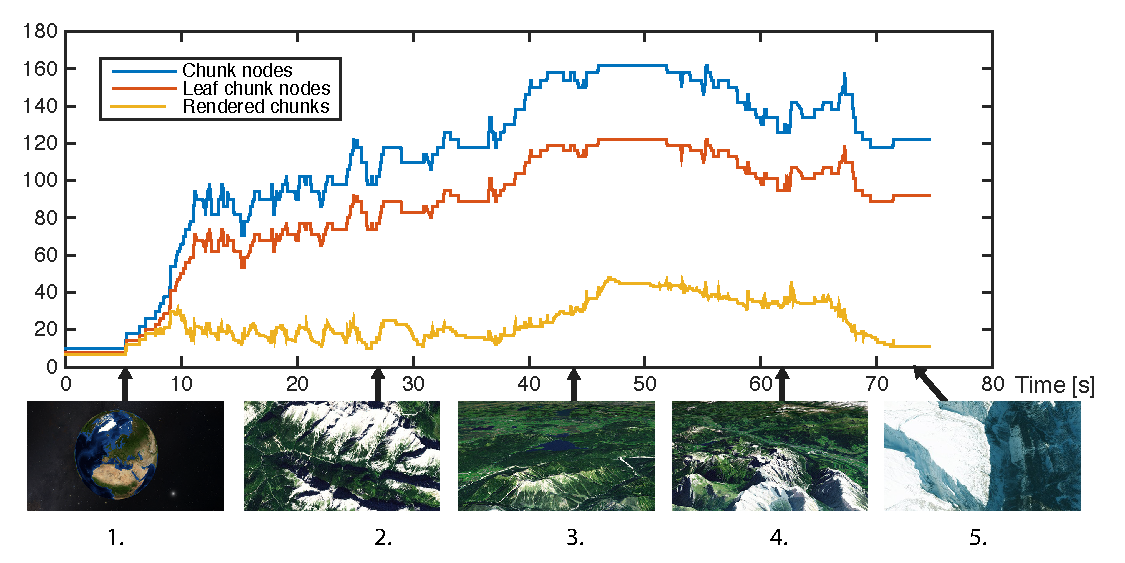
\includegraphics[width=\textwidth]{figures/results/globebrowsing.pdf}
    \end{subfigure}
    \caption{Chunk tree over time when browsing the globe}
    \label{fig:interaction}
\end{figure}

\subsection{Camera Space Rendering}

Comparing the use of camera space rendering and model space rendering, vertex jittering is apparent when interacting close to the surface. Figure \ref{fig:camspacemodelspace} shows how vertex jittering is apparent when browsing a HiRISE patch close to the surface of Mars. The visual result in the image is not as striking as the artifact that appears when the camera is moving. Then the vertices are jittering only in the case of model space rendering and not for camera space rendering. 

\begin{figure}[h]
    \centering
    \begin{subfigure}[bt]{0.48\textwidth}
        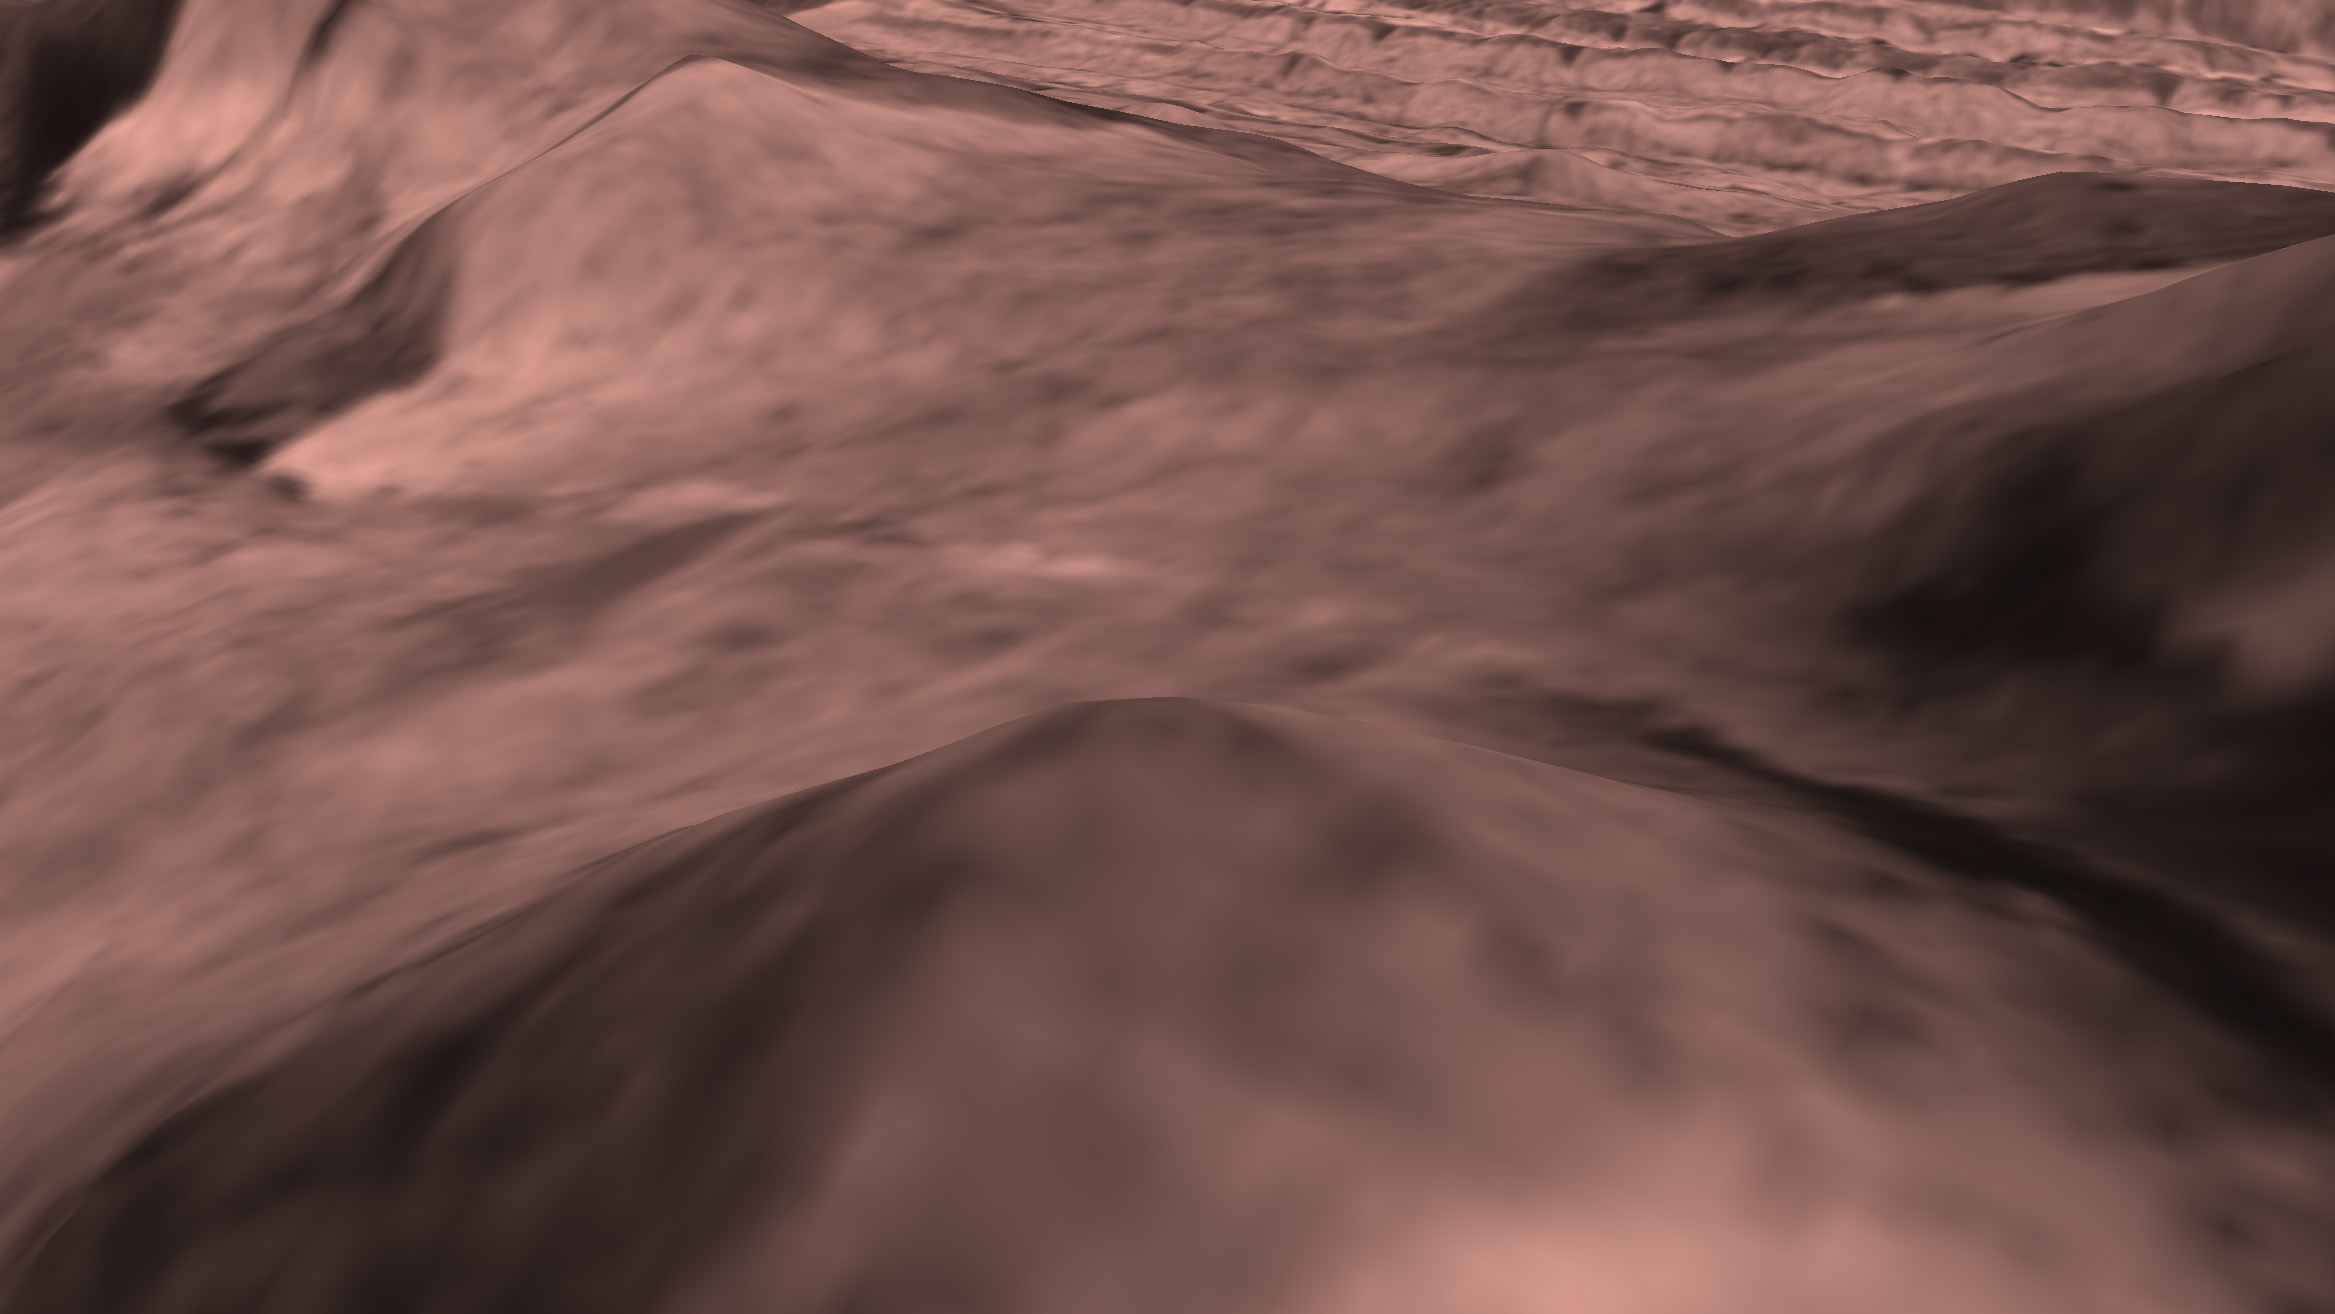
\includegraphics[width=\textwidth]{figures/results/camspace.jpg}
        \caption{Camera space rendering}
    \end{subfigure}
    \begin{subfigure}[bt]{0.48\textwidth}
        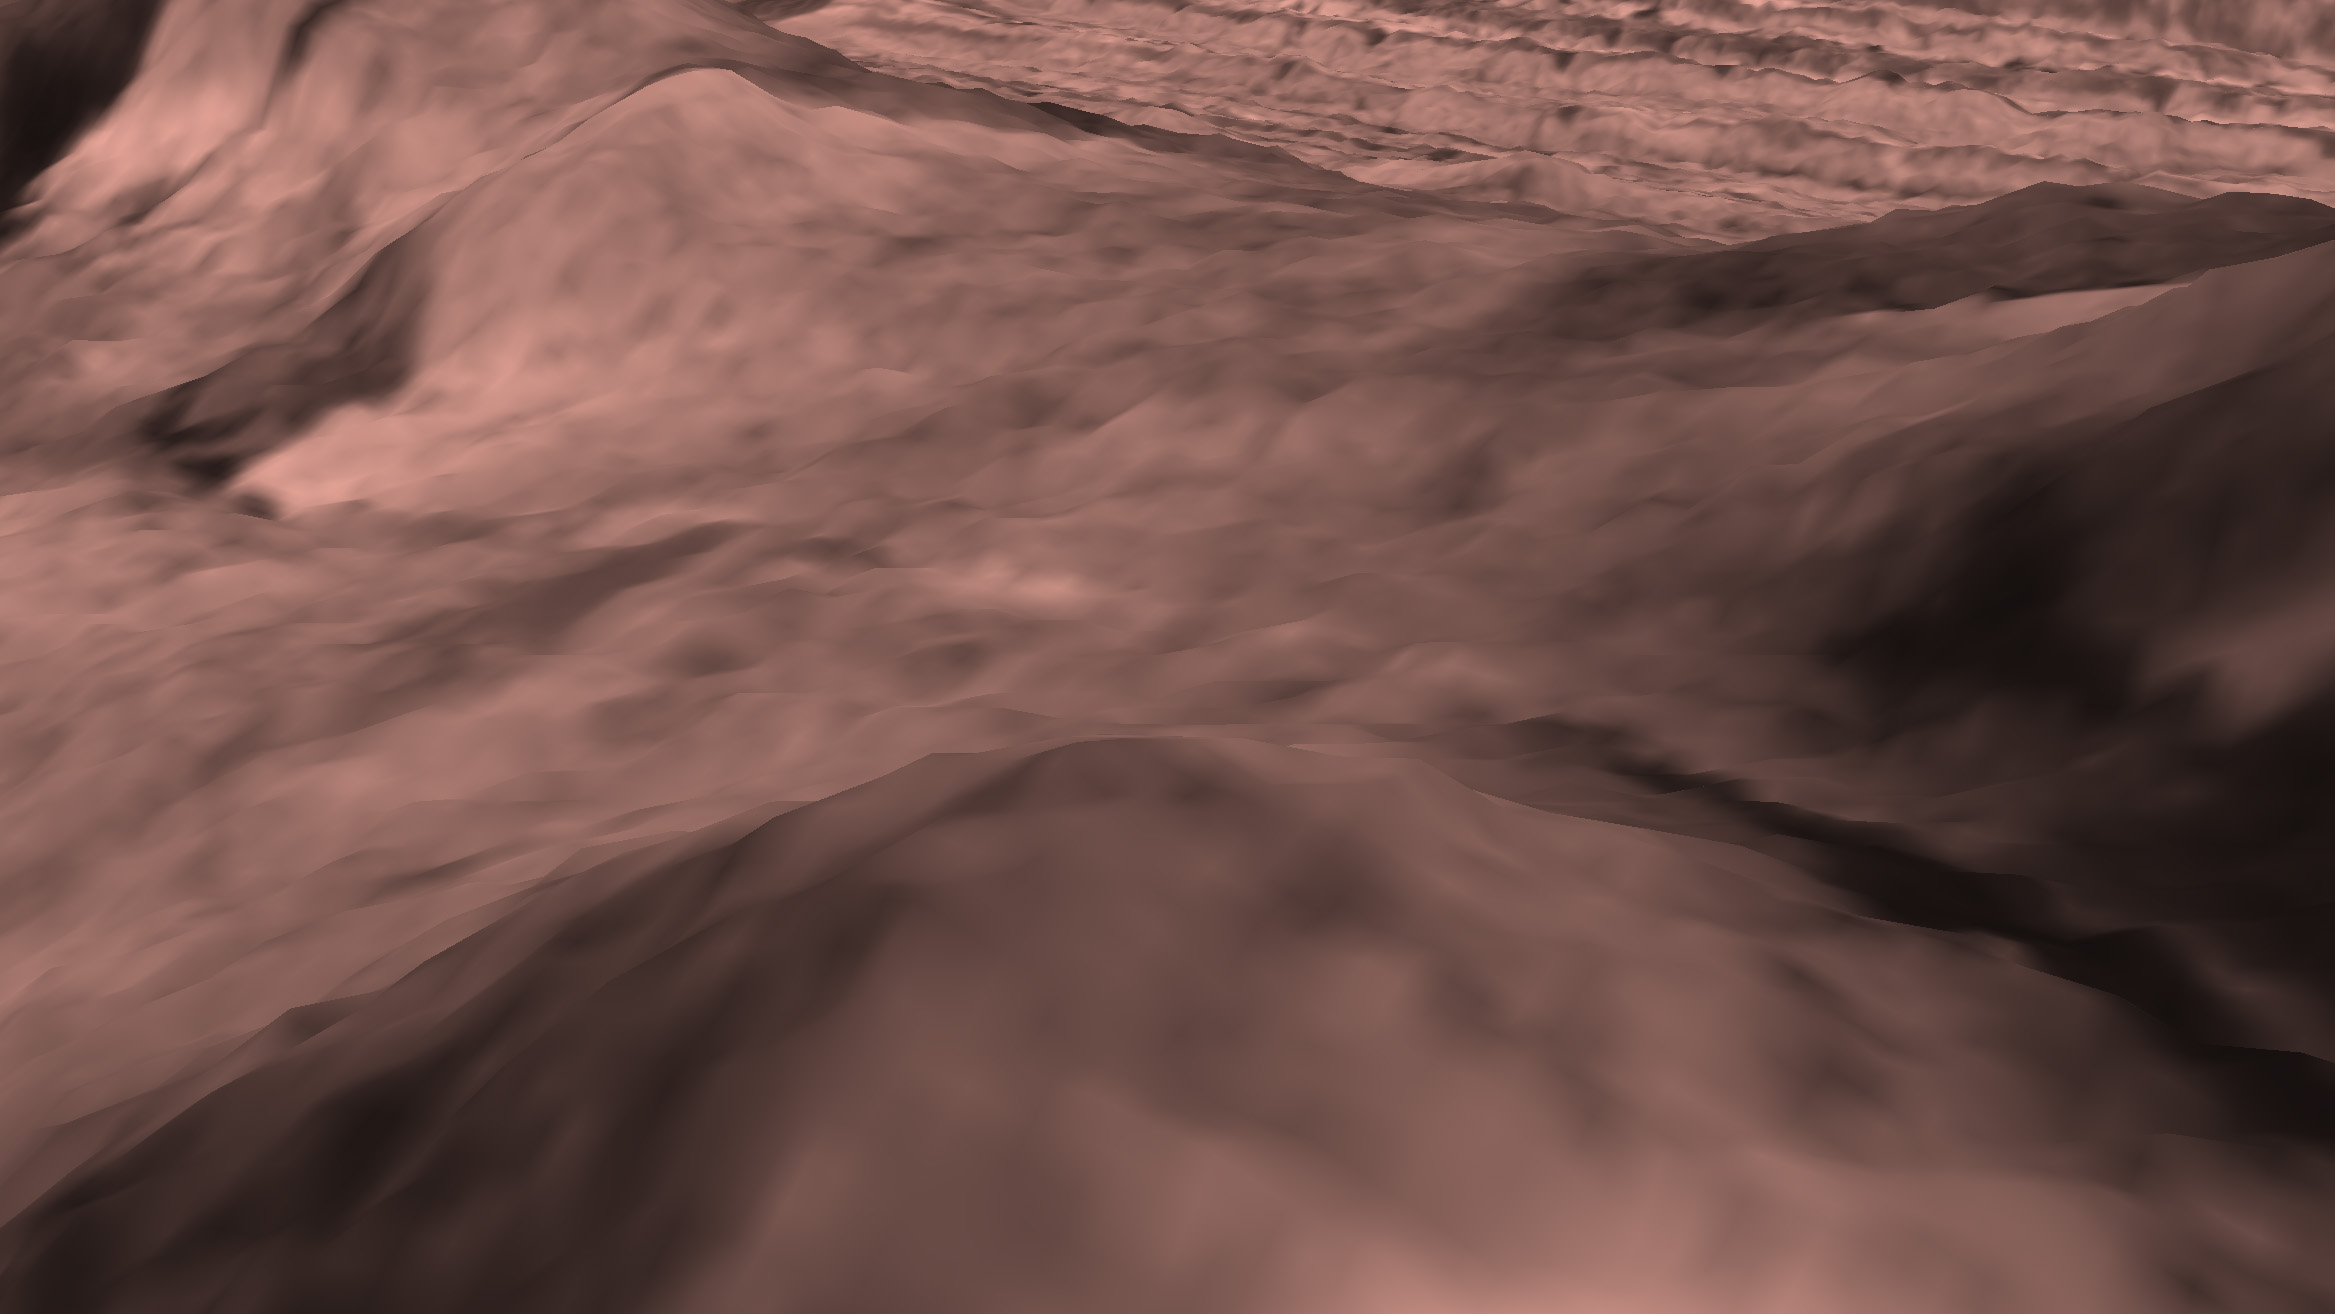
\includegraphics[width=\textwidth]{figures/results/modelspace.jpg}
        \caption{Model space rendering}
    \end{subfigure}
    \caption{Vertex jittering of model space rendering}
    \label{fig:camspacemodelspace}
\end{figure}


\FloatBarrier
